\documentclass{tufte-book}

\hypersetup{colorlinks}% uncomment this line if you prefer colored hyperlinks (e.g., for onscreen viewing)

%%
% Book metadata
\title{The BlackBook}
\author[The Black family]{The Black family}
\publisher{The Black family recipe book, typeset by James}

%%
% If they're installed, use Bergamo and Chantilly from www.fontsite.com.
% They're clones of Bembo and Gill Sans, respectively.
%\IfFileExists{bergamo.sty}{\usepackage[osf]{bergamo}}{}% Bembo
%\IfFileExists{chantill.sty}{\usepackage{chantill}}{}% Gill Sans

%\usepackage{microtype}

%%
% Just some sample text
\usepackage{lipsum}

%%
% For nicely typeset tabular material
\usepackage{booktabs}


%%
% For graphics / images
\usepackage{graphicx}
\setkeys{Gin}{width=\linewidth,totalheight=\textheight,keepaspectratio}
\graphicspath{{graphics/}}

% The fancyvrb package lets us customize the formatting of verbatim
% environments.  We use a slightly smaller font.
\usepackage{fancyvrb}
\fvset{fontsize=\normalsize}

%%
% Prints argument within hanging parentheses (i.e., parentheses that take
% up no horizontal space).  Useful in tabular environments.
\newcommand{\hangp}[1]{\makebox[0pt][r]{(}#1\makebox[0pt][l]{)}}

%%
% Prints an asterisk that takes up no horizontal space.
% Useful in tabular environments.
\newcommand{\hangstar}{\makebox[0pt][l]{*}}

%%
% Prints a trailing space in a smart way.
\usepackage{xspace}

%%
% Some shortcuts for Tufte's book titles.  The lowercase commands will
% produce the initials of the book title in italics.  The all-caps commands
% will print out the full title of the book in italics.
\newcommand{\vdqi}{\textit{VDQI}\xspace}
\newcommand{\ei}{\textit{EI}\xspace}
\newcommand{\ve}{\textit{VE}\xspace}
\newcommand{\be}{\textit{BE}\xspace}
\newcommand{\VDQI}{\textit{The Visual Display of Quantitative Information}\xspace}
\newcommand{\EI}{\textit{Envisioning Information}\xspace}
\newcommand{\VE}{\textit{Visual Explanations}\xspace}
\newcommand{\BE}{\textit{Beautiful Evidence}\xspace}

\newcommand{\TL}{Tufte-\LaTeX\xspace}

% Prints the month name (e.g., January) and the year (e.g., 2008)
\newcommand{\monthyear}{%
  \ifcase\month\or January\or February\or March\or April\or May\or June\or
  July\or August\or September\or October\or November\or
  December\fi\space\number\year
}


% Prints an epigraph and speaker in sans serif, all-caps type.
\newcommand{\openepigraph}[2]{%
  %\sffamily\fontsize{14}{16}\selectfont
  \begin{fullwidth}
  \sffamily\large
  \begin{doublespace}
  \noindent\allcaps{#1}\\% epigraph
  \noindent\allcaps{#2}% author
  \end{doublespace}
  \end{fullwidth}
}

% Inserts a blank page
\newcommand{\blankpage}{\newpage\hbox{}\thispagestyle{empty}\newpage}

\usepackage{units}

% Typesets the font size, leading, and measure in the form of 10/12x26 pc.
\newcommand{\measure}[3]{#1/#2$\times$\unit[#3]{pc}}

% Macros for typesetting the documentation
\newcommand{\hlred}[1]{\textcolor{Maroon}{#1}}% prints in red
\newcommand{\hangleft}[1]{\makebox[0pt][r]{#1}}
\newcommand{\hairsp}{\hspace{1pt}}% hair space
\newcommand{\hquad}{\hskip0.5em\relax}% half quad space
\newcommand{\TODO}{\textcolor{red}{\bf TODO!}\xspace}
\newcommand{\ie}{\textit{i.\hairsp{}e.}\xspace}
\newcommand{\eg}{\textit{e.\hairsp{}g.}\xspace}
\newcommand{\na}{\quad--}% used in tables for N/A cells
\providecommand{\XeLaTeX}{X\lower.5ex\hbox{\kern-0.15em\reflectbox{E}}\kern-0.1em\LaTeX}
\newcommand{\tXeLaTeX}{\XeLaTeX\index{XeLaTeX@\protect\XeLaTeX}}
% \index{\texttt{\textbackslash xyz}@\hangleft{\texttt{\textbackslash}}\texttt{xyz}}
\newcommand{\tuftebs}{\symbol{'134}}% a backslash in tt type in OT1/T1
\newcommand{\doccmdnoindex}[2][]{\texttt{\tuftebs#2}}% command name -- adds backslash automatically (and doesn't add cmd to the index)
\newcommand{\doccmddef}[2][]{%
  \hlred{\texttt{\tuftebs#2}}\label{cmd:#2}%
  \ifthenelse{\isempty{#1}}%
    {% add the command to the index
      \index{#2 command@\protect\hangleft{\texttt{\tuftebs}}\texttt{#2}}% command name
    }%
    {% add the command and package to the index
      \index{#2 command@\protect\hangleft{\texttt{\tuftebs}}\texttt{#2} (\texttt{#1} package)}% command name
      \index{#1 package@\texttt{#1} package}\index{packages!#1@\texttt{#1}}% package name
    }%
}% command name -- adds backslash automatically
\newcommand{\doccmd}[2][]{%
  \texttt{\tuftebs#2}%
  \ifthenelse{\isempty{#1}}%
    {% add the command to the index
      \index{#2 command@\protect\hangleft{\texttt{\tuftebs}}\texttt{#2}}% command name
    }%
    {% add the command and package to the index
      \index{#2 command@\protect\hangleft{\texttt{\tuftebs}}\texttt{#2} (\texttt{#1} package)}% command name
      \index{#1 package@\texttt{#1} package}\index{packages!#1@\texttt{#1}}% package name
    }%
}% command name -- adds backslash automatically
\newcommand{\docopt}[1]{\ensuremath{\langle}\textrm{\textit{#1}}\ensuremath{\rangle}}% optional command argument
\newcommand{\docarg}[1]{\textrm{\textit{#1}}}% (required) command argument
\newenvironment{docspec}{\begin{quotation}\ttfamily\parskip0pt\parindent0pt\ignorespaces}{\end{quotation}}% command specification environment
\newcommand{\docenv}[1]{\texttt{#1}\index{#1 environment@\texttt{#1} environment}\index{environments!#1@\texttt{#1}}}% environment name
\newcommand{\docenvdef}[1]{\hlred{\texttt{#1}}\label{env:#1}\index{#1 environment@\texttt{#1} environment}\index{environments!#1@\texttt{#1}}}% environment name
\newcommand{\docpkg}[1]{\texttt{#1}\index{#1 package@\texttt{#1} package}\index{packages!#1@\texttt{#1}}}% package name
\newcommand{\doccls}[1]{\texttt{#1}}% document class name
\newcommand{\docclsopt}[1]{\texttt{#1}\index{#1 class option@\texttt{#1} class option}\index{class options!#1@\texttt{#1}}}% document class option name
\newcommand{\docclsoptdef}[1]{\hlred{\texttt{#1}}\label{clsopt:#1}\index{#1 class option@\texttt{#1} class option}\index{class options!#1@\texttt{#1}}}% document class option name defined
\newcommand{\docmsg}[2]{\bigskip\begin{fullwidth}\noindent\ttfamily#1\end{fullwidth}\medskip\par\noindent#2}
\newcommand{\docfilehook}[2]{\texttt{#1}\index{file hooks!#2}\index{#1@\texttt{#1}}}
\newcommand{\doccounter}[1]{\texttt{#1}\index{#1 counter@\texttt{#1} counter}}

% Generates the index
%\usepackage{makeidx}
\usepackage[makeindex, split]{splitidx}

\makeindex
\newindex[Recipes]{recipe}

\usepackage{ gensymb } % for celcius


\begin{document}

% Front matter
\frontmatter

% r.1 blank page
%\blankpage

% v.2 epigraphs
\newpage\thispagestyle{empty}
\openepigraph{%
Is there that owre his French ragout,
Or olio that wad staw a sow,
Or fricassee wad mak her spew
Wi perfect scunner,
Looks down wi sneering, scornfu view
On sic a dinner?
}{Robbie Burns, \emph{Address to a Haggis}%, {\itshape Design, Form, and Chaos}
}
\vfill
\openepigraph{%
After a good dinner one can forgive anybody, even one's own relations.
}{Oscar Wilde, \emph{A Woman of No Importance}}
\vfill
\openepigraph{%
Let food be thy medicine and medicine be thy food.
}{Hippocrates}
\vfill
\openepigraph{%
Training is everything. The peach was once a bitter almond; cauliflower is nothing but cabbage with a college education.
}{Mark Twain}
\vfill
\openepigraph{%
Vegetarians, and their Hezbollah-like splinter faction, the vegans ... are the enemy of everything good and decent in the human spirit.
}{Anthony Bourdain, \emph{Kitchen Confidential}}

% r.3 full title page
\maketitle


% v.4 copyright page
\newpage
\begin{fullwidth}
~\vfill
\thispagestyle{empty}
\setlength{\parindent}{0pt}
\setlength{\parskip}{\baselineskip}
Copyright \copyright\ \the\year\ \thanklessauthor

\par\smallcaps{This is \thanklesspublisher}

\par\smallcaps{The tastiest recipes, all vetted by Bill}

\par The majority of these recipes are from Bill's recipe notebook, which is a continuos document, that he has curated over many years. He makes no claim to inventing the recipe, but every recipe has been meticulously tested. This book is designed to be written, and updated. Much like the original notebook this recipe book is based off. Unless required by applicable law or agreed to in writing, recipes distributed here are on a \smallcaps{``AS IS'' BASIS, WITHOUT WARRANTIES OR CONDITIONS OF ANY KIND}, either express or implied. We take responsibility for any kitchen disasters that you may experience.

\par\textit{A continuos document, \monthyear}
\end{fullwidth}

% r.5 contents
\cleardoublepage
\tableofcontents

%\listoffigures
%\listoftables

% r.7 dedication
\cleardoublepage
~\vfill
\begin{doublespace}
\noindent\fontsize{18}{22}\selectfont\itshape
\nohyphenation
Dedicated to Bill Black
\end{doublespace}
\vfill
\vfill


% r.9 introduction
\cleardoublepage
\chapter*{Introduction}

This cookbook is a collaborative work. The majority of the recipes come from Bill's recipe book, which he has collected over many years. Tina and I have added a few of our favourites, and tested out all the recipes in our own kitchen. While Tina took the majority of the photos in this book, you'll have to forgive the less artistic pictures as they were probably my contributions.




%%
% Start the main matter (normal chapters)
\mainmatter

%example four pictures
\begin{figure*}[p]
\fbox{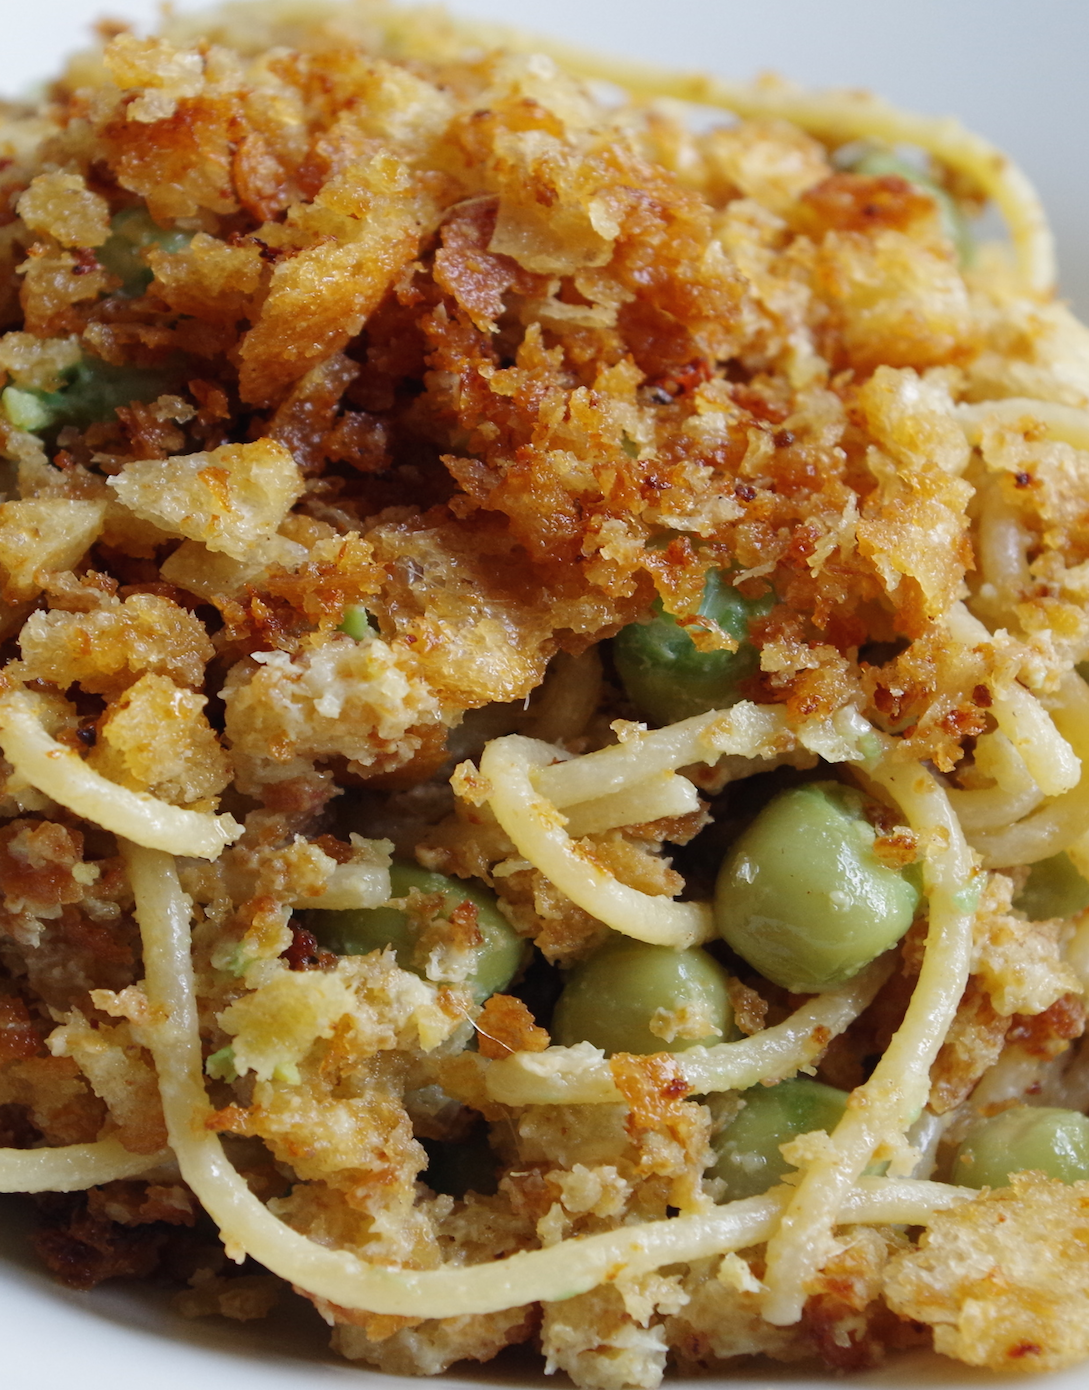
\includegraphics[width=0.45\linewidth,height=0.45\textheight]{graphics/breadcrumb_cover.png}}
\hfill
\fbox{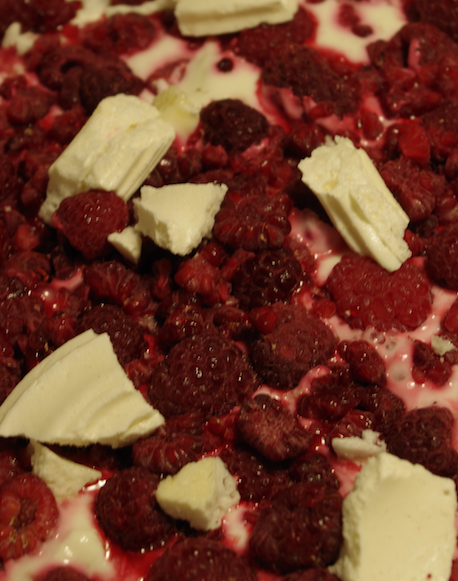
\includegraphics[width=0.45\linewidth,height=0.45\textheight]{graphics/germanmess_cover.png}}
\\\vspace{\baselineskip}
\fbox{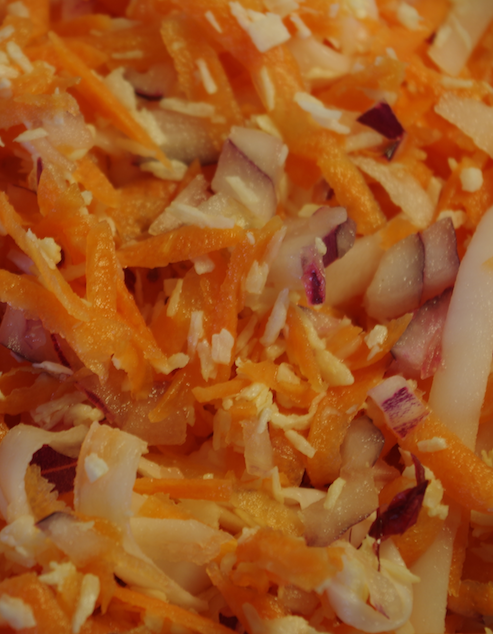
\includegraphics[width=0.45\linewidth,height=0.45\textheight]{graphics/carrotraita_cover.png}}
\hfill
\fbox{
\includegraphics[width=0.45\linewidth,height=0.45\textheight]{graphics/be-title.pdf}}
\end{figure*}

%%%%%%%%%%%%%%%%%%%%%%%%%%%%%%%%%%%%%%%%%
\chapter{Brunch}
%%%%%%%%%%%%%%%%%%%%%%%%%%%%%%%%%%%%%%%%%

\section{Breakfast burritos}
\index{x!x}

NEED TO ADD!

\begin{marginfigure}%
  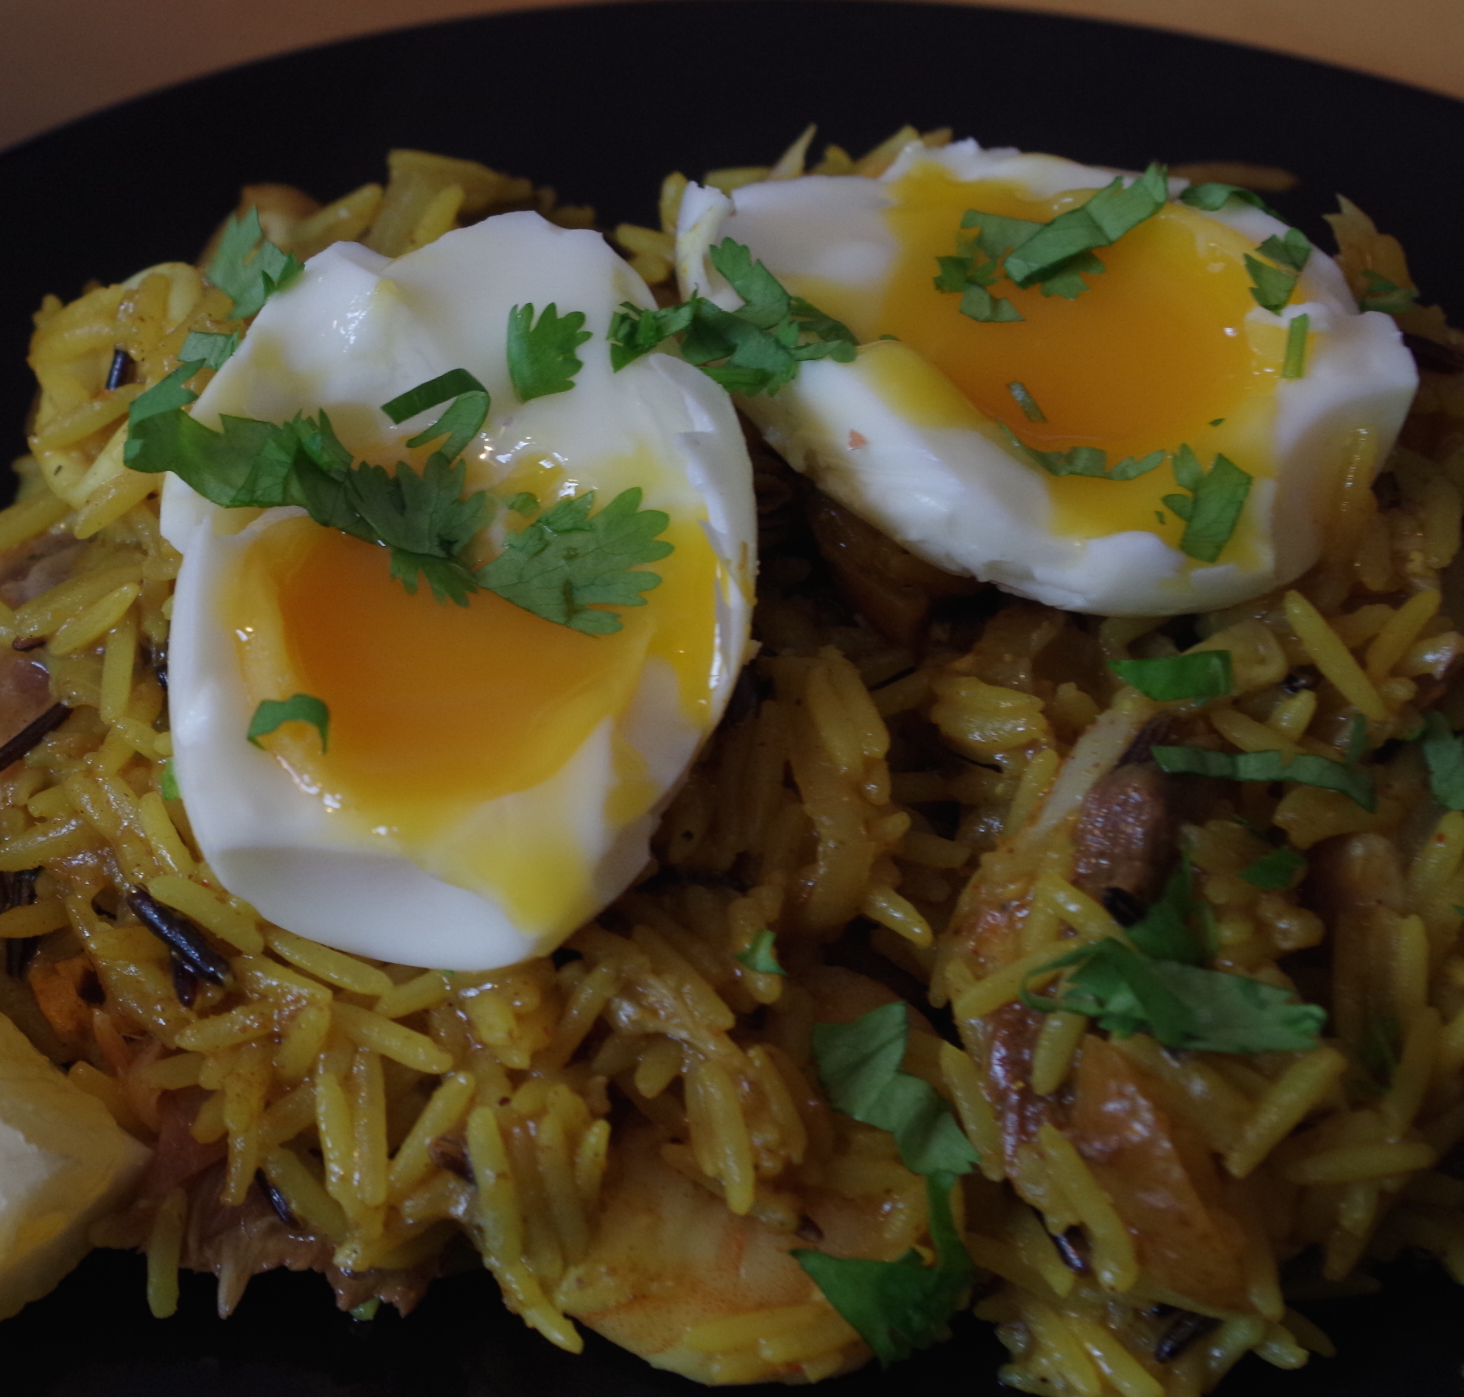
\includegraphics[width=\linewidth]{kedgeree.png}
\end{marginfigure}

\smallskip
\newpart{For rice:}
\\\emph{120g rice
\\1 lemon sliced into quarters
}
\\\newpart{For yoghurt:}
\\\emph{Big handful coriander finely cut
\\Rind of 1 lemon
}
\smallskip
\\Get 600ml of stock to the boil, then add the eggs and set the timer to soft boiled (take eggs out of the stock when they are cooked).

%%%%%%%%%%%%%%%%%%%%%%%%%%%%%%%%%%%%%%%%%

\section{Kedgeree}
\index{Seafood curry!seafood}
\index{Brunch!kedgeree}
\index{Rice!kedgeree}

Not the usual brunch fare, but this colonial throwback can also make an easy dinner. Recipe serves two.

\begin{marginfigure}%
  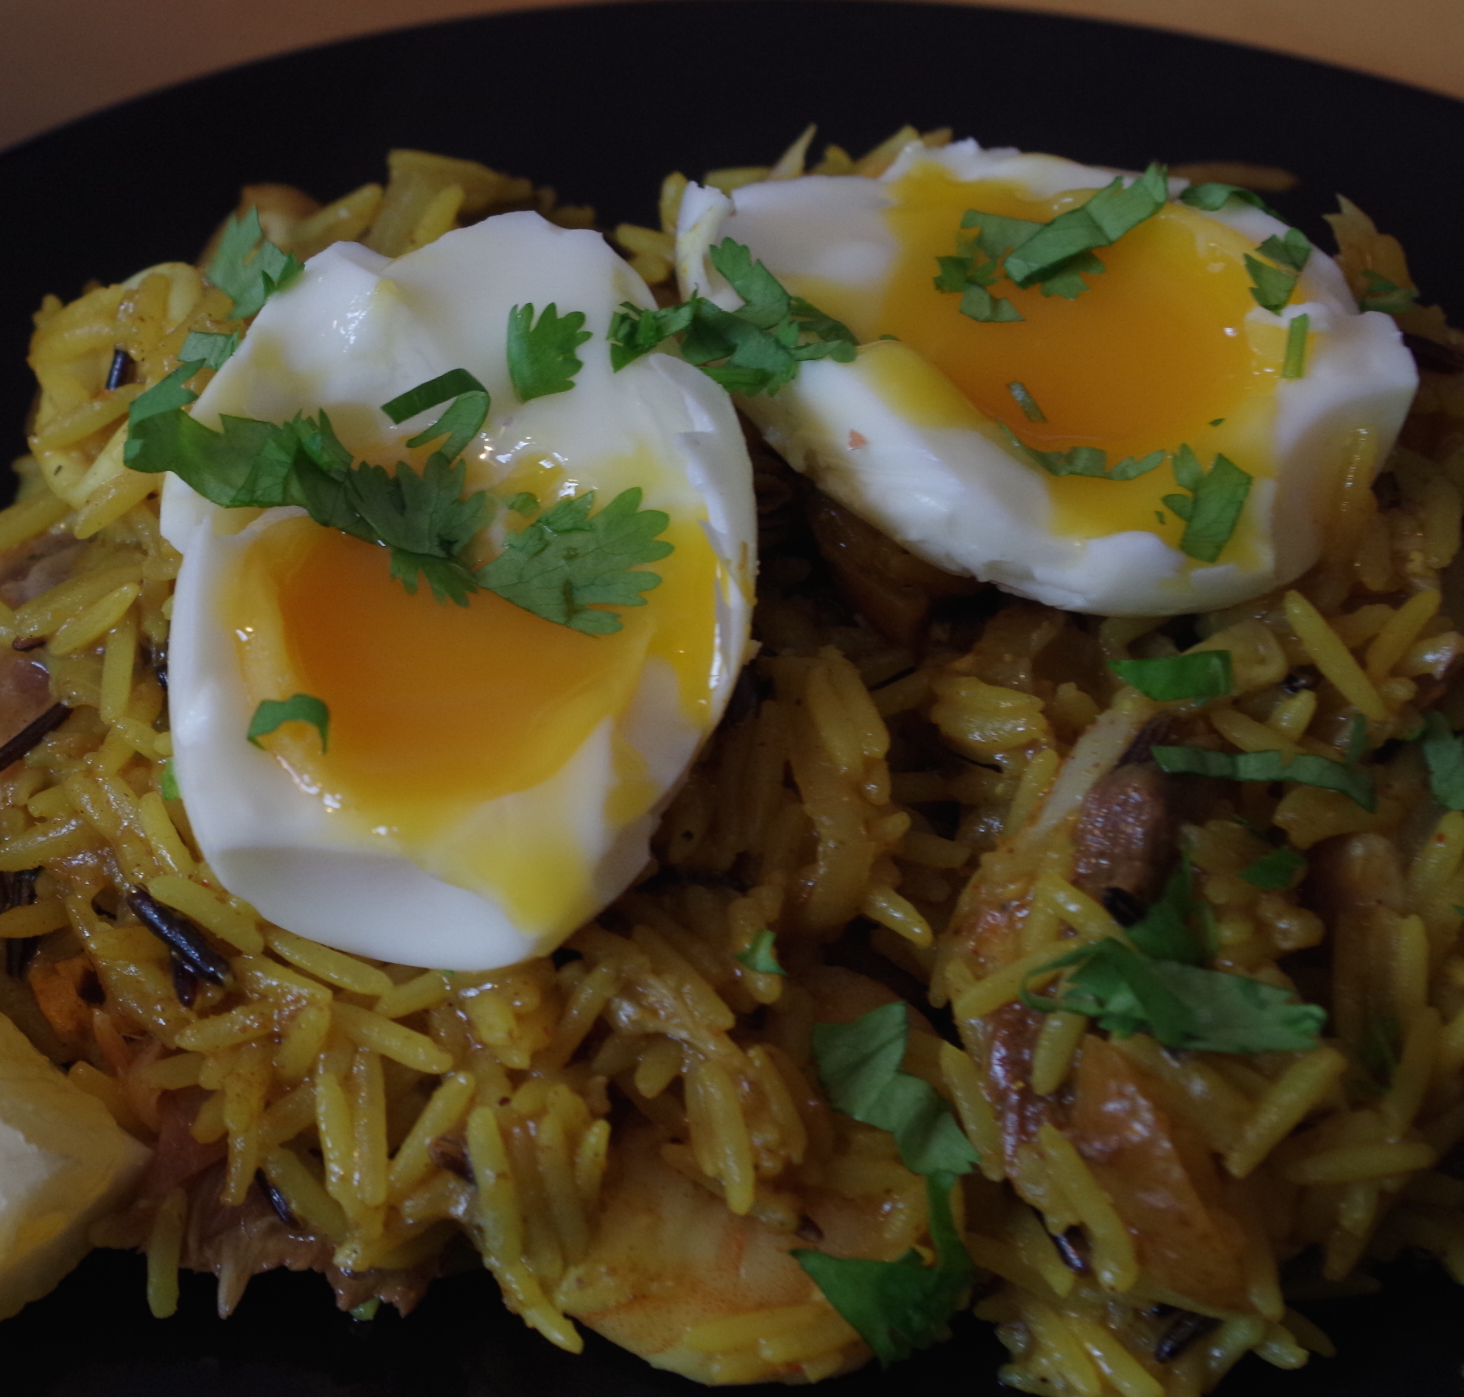
\includegraphics[width=\linewidth]{kedgeree.png}
\end{marginfigure}

\smallskip
\newpart{For rice:}
\\\emph{120g rice
\\600ml stock
\\2 eggs
\\1 onion sliced
\\3 cloves garlic
\\1 tbsp English curry powder
\\1 tsp tumeric
\\5 curry leaves or 3 bay leaves
\\2 fillets smoked fish\sidenote{
In the photo we also added some cooked seafood right before serving.}
\\1 chilli
\\1 tbsp butter
\\1 lemon sliced into quarters
}
\\\newpart{For yoghurt:}
\\\emph{Big handful coriander finely cut
\\1/2 cup yoghurt
\\Rind of 1 lemon
}
\smallskip
\\Get 600ml of stock to the boil, then add the eggs and set the timer to soft boiled (take eggs out of the stock when they are cooked).
\\In another pan, fry the onion with the curry powder, tumeric and a little oil. After a few minutes, add the garlic.
\\Once the onion is starting to brown, add the rice and stir. As soon as it's mixed, add in the stock. 
\\Keep the rice on medium high and occasionally stir. You might need to add a little water.
\\Once the rice is cooked, add in the seafood and butter. Season after tasting, as the fish might be salty. Serve with lemon wedges and sprinkle coriander on as garnish.
\\Mix the yoghurt, rind and coriander. Serve with rice.

Mix lukewarm milk with sugar and yeast. Leave for 10 minutes until you see bubbles. 
Mix butter, flour and salt together. Then add the milk-sugar-yearst mix.
Knead well until dough doesn't stick to your hands anymore.
Let the dough rise (approx. 20 mins in the oven at about 35 degrees).
Then roll dough out on a square tray. Place plums on top. 
Let it rise again (approx. 20 mins in the oven at about 50 degrees).
Then bake for 25 mins at 175 degrees. 
Serve with cream.

%%%%%%%%%%%%%%%%%%%%%%%%%%%%%%%%%%%%%%%%%

\section{Plum cake}
\index{Brunch!plum cake}
\index{Dessert!plum cake}

\begin{marginfigure}%
  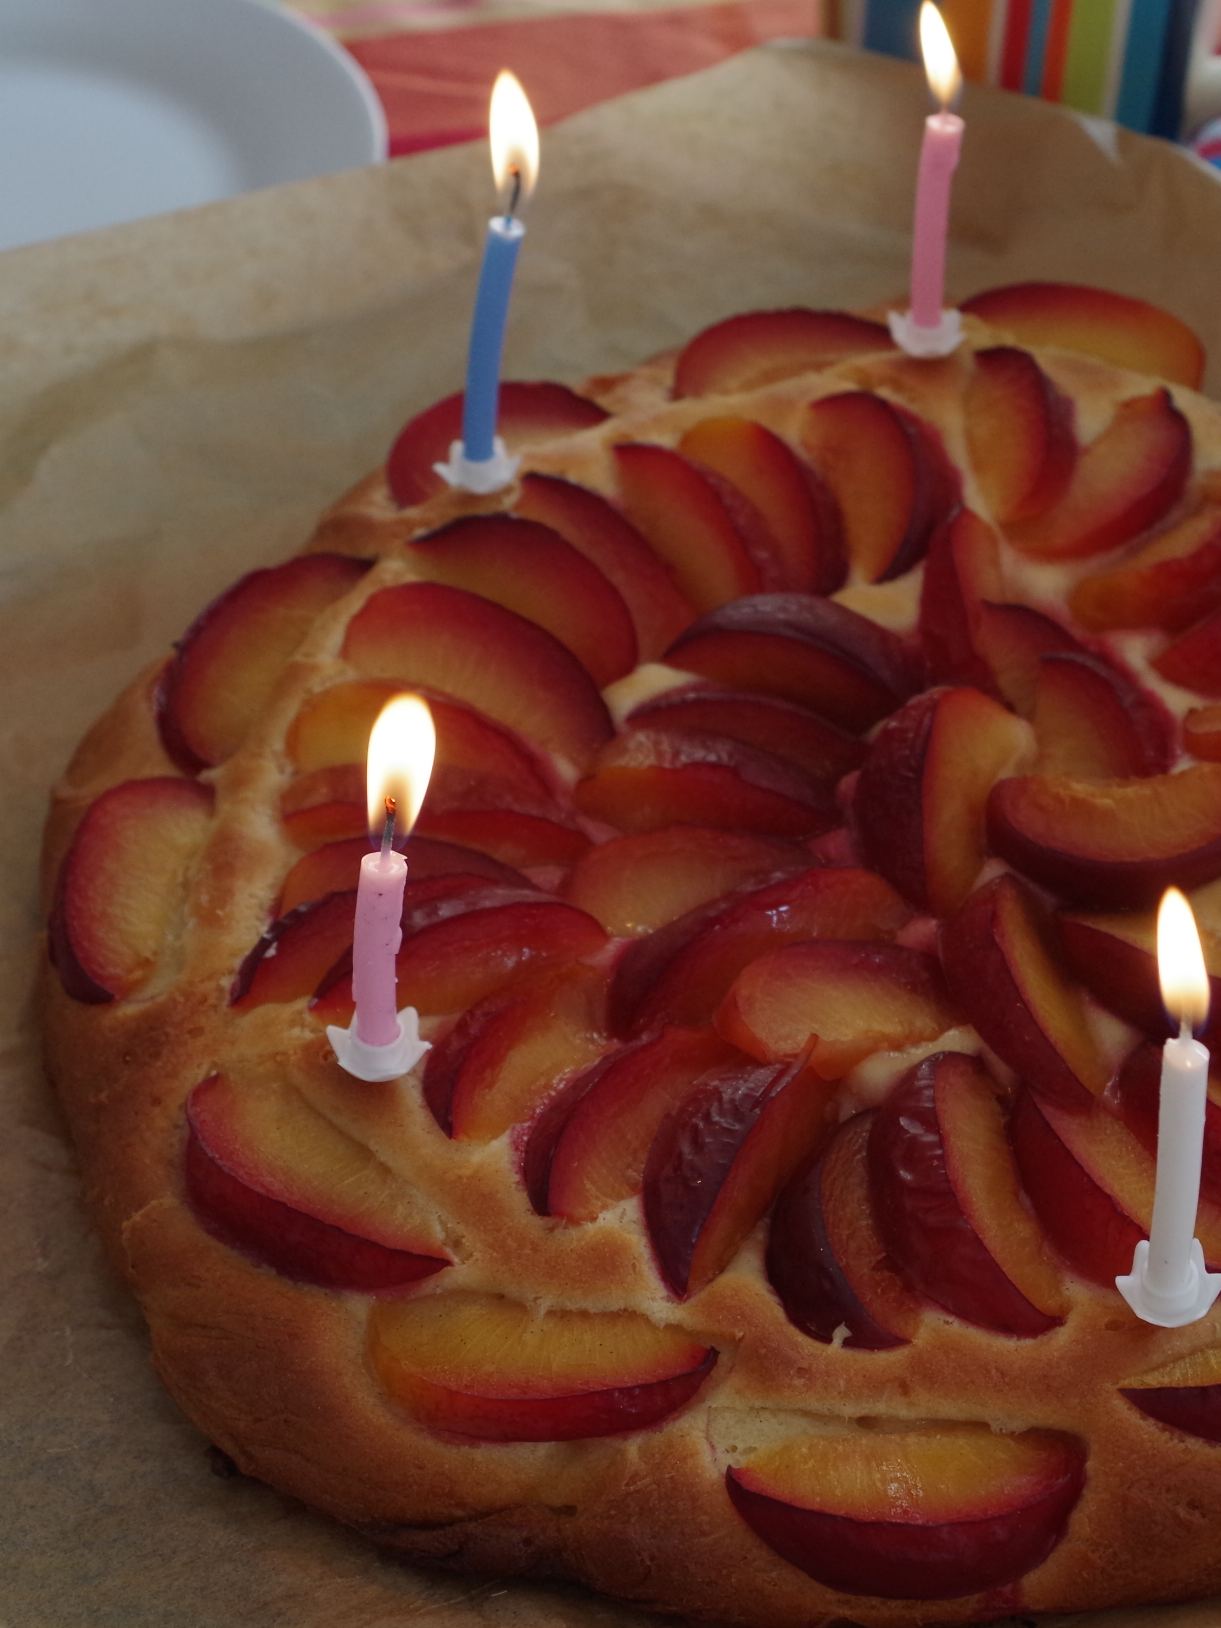
\includegraphics[width=\linewidth]{plumcake.png}
\end{marginfigure}

Plum cake is originally a Bavarian dish, known as Zwetschgendatschi. It's spread throughout Germany, where is it often known as Pflaumenkuchen (literally, "plum cake"). While in Cambridge, Tina and I have made use of the orchards a few miles away from Cambridge at her old college of Girton. In days after a trip to the orchard, our diet switches to mainly plum cake as we eat our way through kilograms and kilograms of the fruit.

\smallskip
\emph{2 sachets yeast (each sachet has 7g)
\\500g flour
\\220g sugar\sidenote{Tina usually uses only 120g}
\\250ml milk
\\100g butter
\\2kg plums
}

\smallskip
Mix lukewarm milk with sugar and yeast. Leave for 10 minutes until you see bubbles. 
\\Mix butter, flour and salt together. Then add the milk-sugar-yearst mix.
\\Knead well until dough doesn't stick to your hands anymore.
\\Let the dough rise (approx. 20 mins in the oven at about 35 degrees).
\\Then roll dough out on a square tray. Place plums on top. 
\\Let it rise again (approx. 20 mins in the oven at about 50 degrees).
\\Then bake for 25 mins at 175 degrees.\sidenote{If the plums are sour, you can also add some more sugar on top before baking).}

%%%%%%%%%%%%%%%%%%%%%%%%%%%%%%%%%%%%%%%%%
\chapter{Starters}
%%%%%%%%%%%%%%%%%%%%%%%%%%%%%%%%%%%%%%%%%
\section{Beetroot hummus}
\index{Starters!beetroot hummus}
\index{Vegetarian!beetroot hummus}
\index{Hummus!beetroot}

I love hummus. This beetroot hummus is a nice twist. If you are motivated to make it extra creamy, you can peel the chick peas. To do this either pinch each check pea one by one, or, to speed things up just put them in a bowl with water and rub the chick peas together. The second method won't get all the skins, but it only takes a few minutes. The hummus also tastes better after sitting overnight in the fridge.

\begin{marginfigure}%
  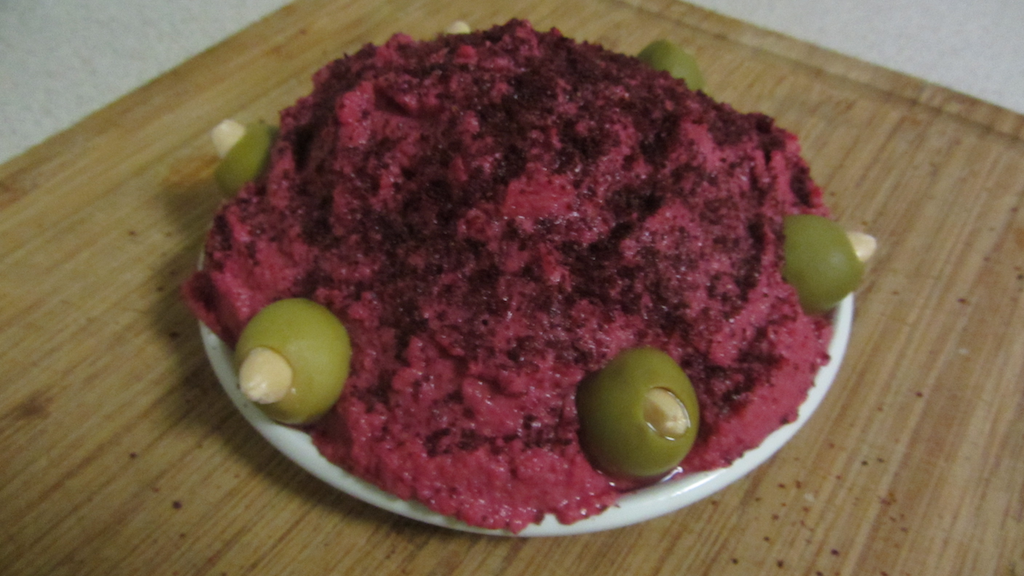
\includegraphics[width=\linewidth]{beetroothummus.png}
\end{marginfigure}

\smallskip
\emph{4 tbsp olive oil
\\1 tin chick peas
\\2 tablespoons tahini
\\2 cloves garlic
\\Large sprinkle toasted cumin seeds
\\4 small cooked beetroot\sidenote{
You can replace with almost anything! My favourite is half a block feta and 4 dates, roughly chopped.}
\\Salt and pepper to taste.
}

\smallskip
Put everything in a food processor.
\\Blitz it, adding water to get the looseness you want. 
\\Serve with sumac and cumin sprinkled on top.

%%%%%%%%%%%%%%%%%%%%%%%%%%%%%%%%%%%%%%%%%
\section{Masala pancakes}
\index{Vegetarian curry!potato pancakes}
\index{Starters!potato pancakes}
\index{Vegetarian!potato pancakes}

A cheats Dosa. While it lacks the fermented taste and super crispy edges of real Dosa, this recipe is a super easy approximation of that South Indian dish. The potato filling and the batter are best made a bit ahead of time.

\begin{marginfigure}%
  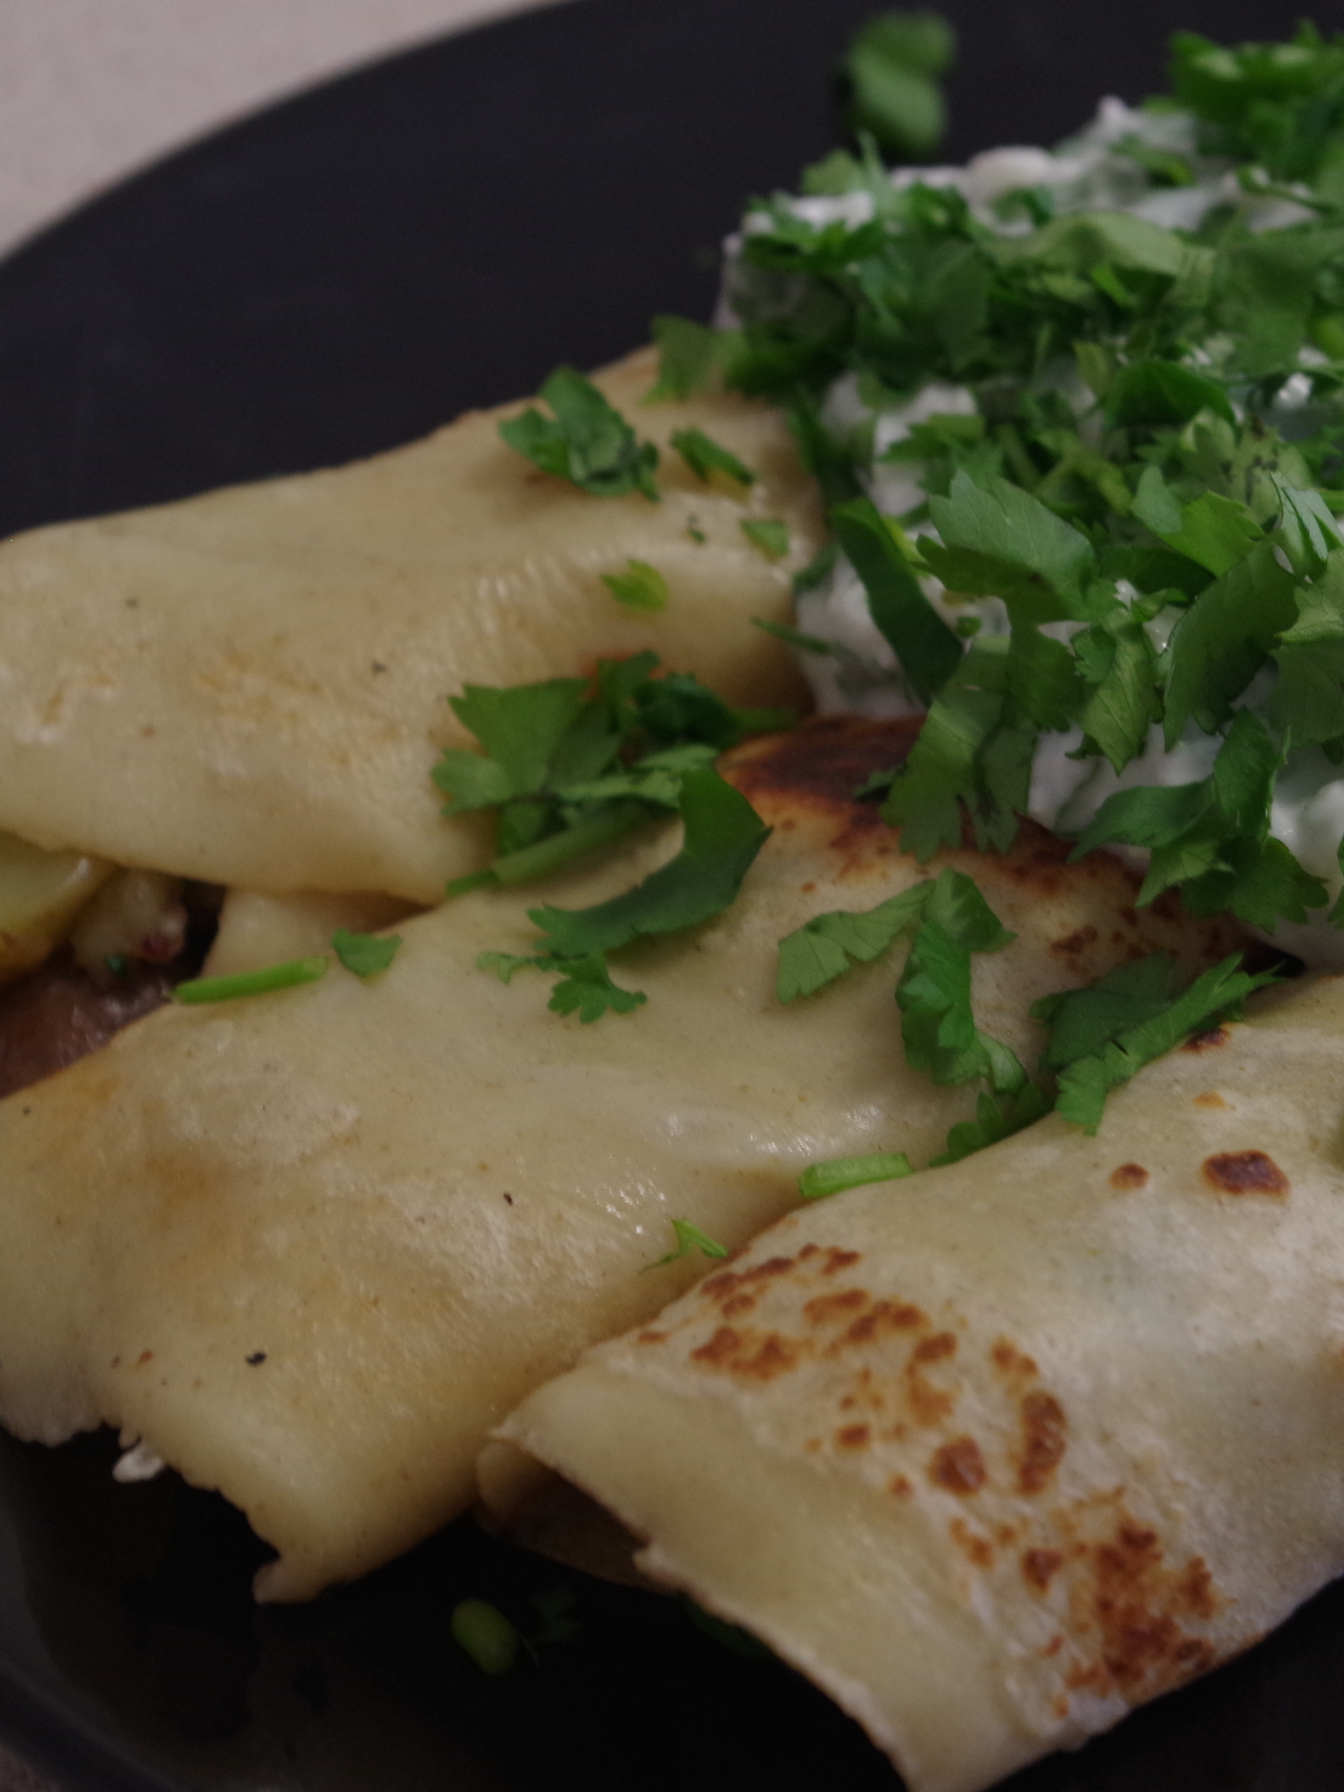
\includegraphics[width=\linewidth]{masalapancakes.png}
\end{marginfigure}

\smallskip
\emph{Olive oil, for frying
\\1 green chilli, deseeded and finely chopped
\\2 garlic cloves, peeled and finely sliced
\\3cm piece of fresh root ginger, peeled and finely chopped
\\125g plain flour
\\1 large egg
\\275ml whole milk
\\1 tsp mustard seeds
\\1/2 onion, peeled and thinly sliced
\\1 tsp ground turmeric
\\4 to 6 cold, peeled boiled potatoes, roughly chopped
\\6 tbsp natural yoghurt
\\2 tbsp chopped coriander}

\smallskip
\newpart{For the potato filling:} 
\\Heat a little oil in a large frying pan over a medium heat, add the mustard seeds and cook for 2 minutes until the seeds begin to pop. Add the onion and cook for 5 minutes until soft and golden brown. Stir in the turmeric and cooked potatoes and season, adding a dash of olive oil if necessary to aid frying. Fry over a medium heat for 4 minutes until softened and heated through. Leave to one side while you cook the pancakes.
\\\newpart{For the pancakes:} 
\\Toast the cumin seeds with a pinch of salt in a dry, medium- hot pan for about 1 minute until aromatic. Add a dash of oil and saute the chilli, garlic and ginger for a further 2 minutes until softened. Remove from the heat.
\\Put the spice/garlic mix into a bowl. Sift in the flour, season and make a well in the middle, then break in the egg and add half of the milk. Whisk the flour into the egg slowly until well incorporated, then gradually add the remaining milk. Continue whisking until the mixture is smooth and has the consistency of double cream. Whisk in 1 teaspoon of oil, then taste and adjust the seasoning if necessary. Leave the batter to rest for 10 minutes.
\\Heat a large, wide frying pan, then add a little oil. If the batter has thickened too much, add a tablespoon or two of milk. Pour in a ladleful of batter and tilt the pan to spread the batter out. Cook for a minute on one side until golden and crisp, then flip the pancake and continue to cook for a further minute until cooked through. Keep warm while repeating with the remaining batter.
\\\newpart{To serve:} 
\\Mix the yoghurt and coriander together and season to taste.
\\To serve, place a large spoonful of the potato filling in the middle of each pancake, adding a dollop of the yoghurt if you like, then roll up into a sausage shape.

%%%%%%%%%%%%%%%%%%%%%%%%%%%%%%%%%%%%%%%%%
\chapter{Sides}
%%%%%%%%%%%%%%%%%%%%%%%%%%%%%%%%%%%%%%%%%
\section{Roast potato with lemon and olives}
\index{Sides!roast potatoes with lemon}
\index{Potato!roasted with lemon and olives}

\smallskip
\emph{4 tbsp olive oil
\\1kg new potatoes, halved
\\1 whole preserved lemon, finely diced
\\4 cloves garlic
\\1 cup pitted olives
\\1/2 cup parsley
}
\smallskip

Pre-heat oven to 200\celsius.
\\Add all ingredients except parsley and mix well.\sidenote{
You can also add in chicken, eggplant, kumera, pumpkin or capsicum}
\\Place in the oven for 45 minutes or until potatoes are tender, slightly shrivelled and browned. 
\\Remove from the oven, toss with parsley and serve.

%%%%%%%%%%%%%%%%%%%%%%%%%%%%%%%%%%%%%%%%%%%%%%%

\section{Parmesan courgette ribbons}
\index{Sides!courgette ribbons}
\index{Courgette!ribbons with parmesan}

\emph{4 tbsp olive oil
\\1kg new potatoes, halved
\\1 whole preserved lemon, finely diced
\\4 cloves garlic
\\1 cup pitted olives
\\1/2 cup parsley
}

\smallskip
Pre-heat oven to 200\celsius.
\\Use vegetable peeler to cut courgette into ribbons.
\\Steam till cooked, then drained.
\\Season with salt and pepper, parmesan and olive oil.

%%%%%%%%%%%%%%%%%%%%%%%%%%%%%%%%%%%%%%%%%
\chapter{Vegetarian}
%%%%%%%%%%%%%%%%%%%%%%%%%%%%%%%%%%%%%%%%%

\section{Buttercup pumpkin, corn and bean stew}
\index{Vegetarian!pumpkin stew}
\index{Pumpkin!stew}

\emph{1 buttercup pumpkin
\\olive oil
\\1 onion finely chopped
\\2 cloves garlic, finely chopped
\\1 tin white beans, drained
\\400g tin of tomatoes, drained
\\Vegetable stock
\\Coriander leaves 
\\1/2 tsp ground cloves  (Or dahl mix instead of these spices)
\\1 1/2 tsp ground cinnamon
\\1 1/2 tsp ground cumin
\\1 1/2 tsp dried oregano
\\1 tsp dried chilli
}

\smallskip
Cut pumpkin in half, scoop out seeds, rub in olive oil on the flesh and place flesh side down on the baking sheet.
\\Roast for 30 minutes in moderate oven.
\\When cool cut into cubes and skin.
\\Sweat onion then add garlic.
\\Add spices, then pumpkin, tomatoes, beans and corn, and just enough stock to cover.
\\Simmer briefly until flavours combine. 
\\Garnish with coriander.

%%%%%%%%%%%%%%%%%%%%%%%%%%%%%%%%%%%%%%%%%


\section{Couscous with spinach, almonds and feta}
\index{Vegetarian!couscous with spinach, feta and almonds}
\index{Spinach!couscous, feta and almonds}

\emph{1 cup couscous
\\1 cup vege stock
\\olive oil
\\Large handful spinach
\\100g feta chopped
\\1 onion, finely chopped
\\3 tbsp slivered almonds
\\zest of one lemon
\\1/2 cup sultanas
\\Greek yoghurt to serve
}

\smallskip
Prepare the couscous with the stock.
\\Saute onions with oil for 4 minutes.
\\Add almonds and zest till nuts start to brown. At the last minute add spinach.\sidenote{
This is super flexible. In the picture, we replaced spinach with beetroot and mushrooms}
\\Fluff up couscous, add onion, cheese and sultanas.
\\Serve with yoghurt.

%%%%%%%%%%%%%%%%%%%%%%%%%%%%%%%%%%%%%%%%%


\section{Spinach, blue cheese and pear salad}
\index{Vegetarian!spinach, blue cheese and pear salad}
\index{Salads!spinach, blue cheese and pear salad}
\index{Spinach!blue cheese and pear salad}
\index{Blue cheese!spinach and pear salad}

A Roquefort salad, without having to have the roquefort. In Cambridge, Shopshire Blue (which is an orange cheese with blue veins) makes a great substitution.

\smallskip
\emph{3 rinsed pears, cut into chunks
\\200g baby spinach
\\1/2 cup blue cheese\sidenote{
I also really like this salad with a strong goats cheese.}
\\1/2 cup toasted walnuts
\\Lemon juice
\\4 tbsp olive oil
\\1/2 tsp honey
\\1 tbsp balsamic vinegar
\\Parmesan shavings
}

\smallskip
Splash the cut pears with lemon juice to prevent them browning.
\\Whisk together the olive oil, balsamic vinegar and honey to make a vinaigrette.
\\Season the vinaigrette, remembering to underseason if the cheese is salty.
\\Fold together all the ingredients except the parmesan and walnuts, which get scattered on when serving.

%%%%%%%%%%%%%%%%%%%%%%%%%%%%%%%%%%%%%%%%%
\chapter{Mains}
%%%%%%%%%%%%%%%%%%%%%%%%%%%%%%%%%%%%%%%%%

\begin{figure*}[h]
  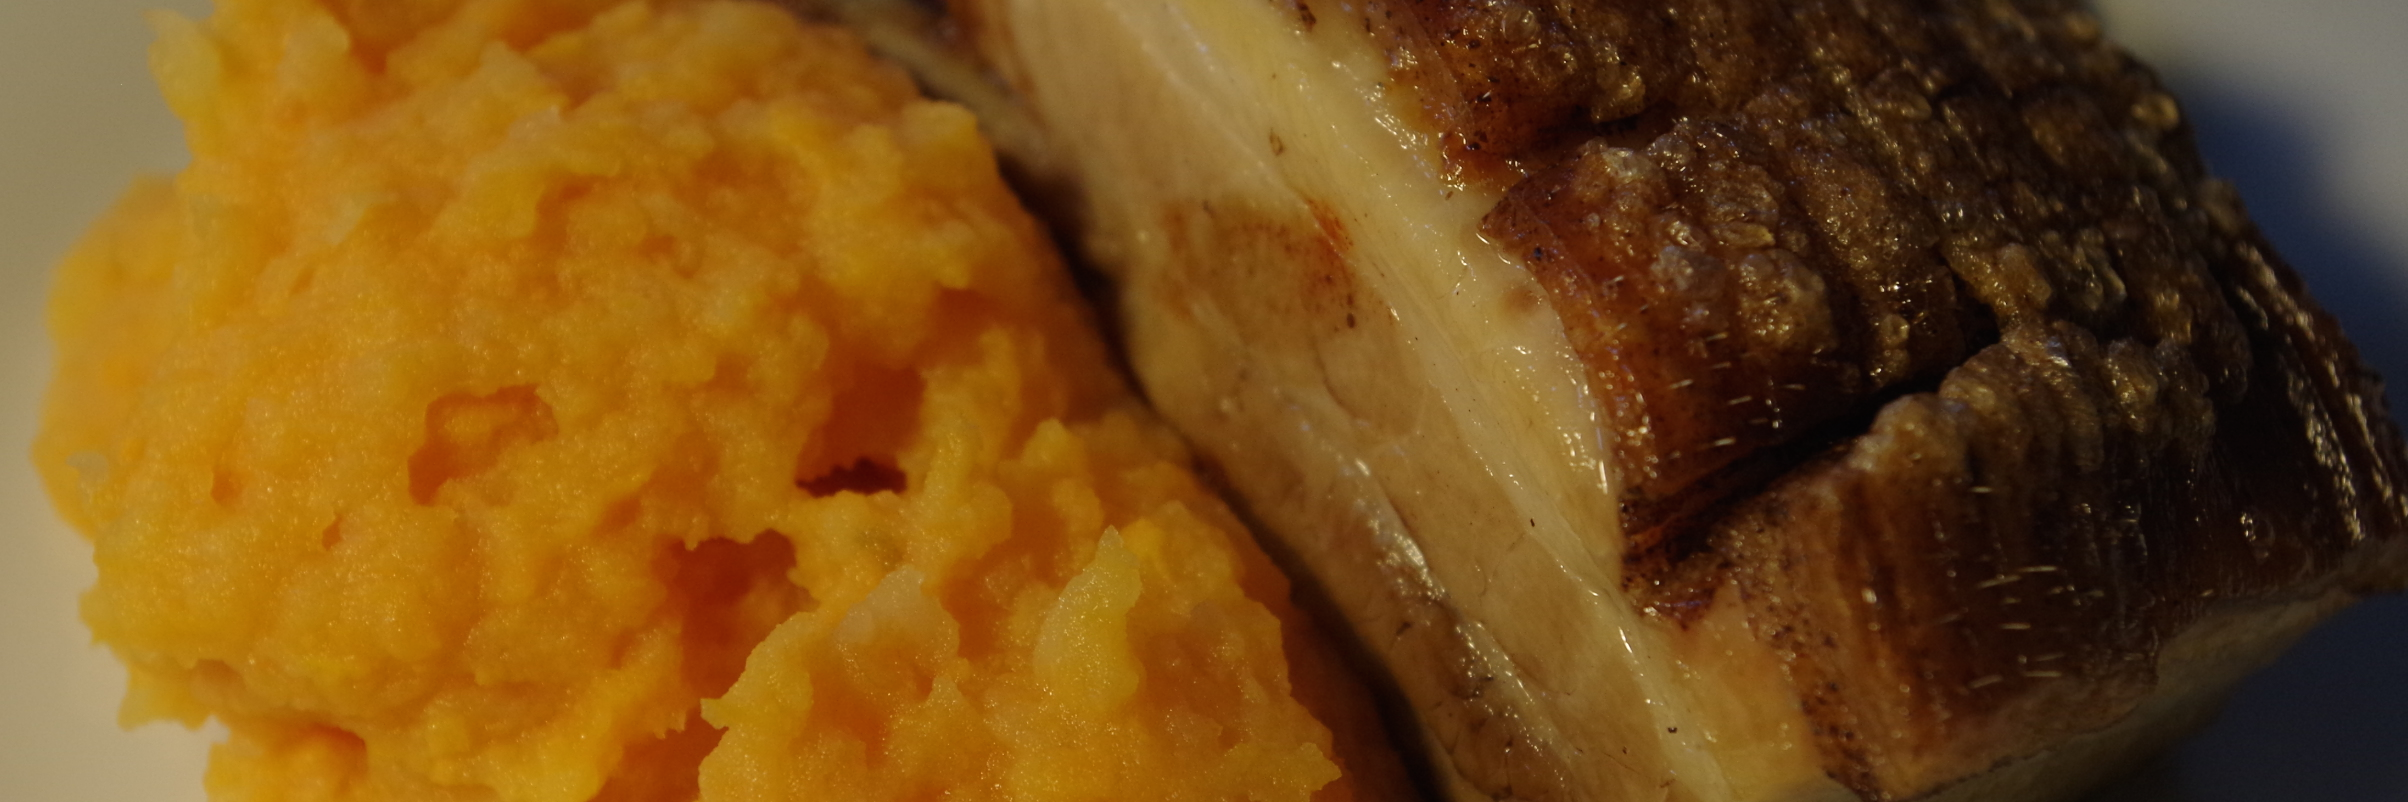
\includegraphics[width=\linewidth]{bellyporkwide.png}
\end{figure*}

\section{Roast pork belly with apple and sweet potato mash}
\index{Mains!Roast pork belly}
\index{Roast!Pork belly}

This dish takes about three days - but it's actually a really easy, and impressive, main to make. This recipe is a slightly modified version of one by Peter Gordon (a kiwi chef). The pork is first marinated, then cooked. It can be served immediately after the first roasting, but if you're cooking it for a dinner party, it can be cooled, portioned into perfect rectangles, then reheated on the day.

\smallskip
\emph{2 kg boneless pork belly
\\50g (5 tbsp) five-spice
\\5 large carrots
\\3 granny-smith apples, peeled and diced
\\700g potatoes, peeled and diced
\\700g sweet potato, peeled and diced
\\50g butter
\\4 tbsp grain mustard
\\2 limes
\\3 tbsp capers, drained and chopped
\\Big bunch of coriander, chopped
}

\smallskip
Score the rind and fat about 1cm apart, being careful to not cut all the way down into the meat. 
\\Mix the five-spice with an equal amount of salt and rub into the pork. Then place the pork in a tupperware so it's just submerged in water and leave for 24-48 hours in the fridge.
\\After the brining has finished, heat the oven to 190\celsius. Place a sheet of baking paper on a rimmed tray, and place the carrots, cut in half long-ways, on top. 
\\Place the pork on top of the carrots, skin side up. Pour 200ml of water on the tray, and roast the pork and carrots for 2 hours. 
\\After two hours, remove the pork and place in the fridge. Keep the fat and carrots as well. At this stage the pork can be kept for up to 4 days.
\\On the day you plan to eat, turn the oven to 190\celsius. 
\\To make the coriander mustard, simply mix lime juice, mustard, capers and coriander. Add a little oil if you want it smoother. 
\\To make the mash, take the fat and and add to a pan with the butter. When the butter starts to brown, add in the apples and carrots and cook with the lid on low till the apple turns to mush. 
\\While the apple cooks, boil the diced potato and sweet potatoes. Once the potatoes are ready, add the apple and mash. This mash can be made a bit early, and reheated when needed. 
\\About 40 minutes before you want to eat, fry the portioned belly pork in a pan with oil till the skin get's bubbly. Then flip the pork over, and put in the oven for 30 minutes.

%%%%%%%%%%%%%%%%%%%%%%%%%%%%%%%%%%%%%%%%%

\begin{figure*}[h]
  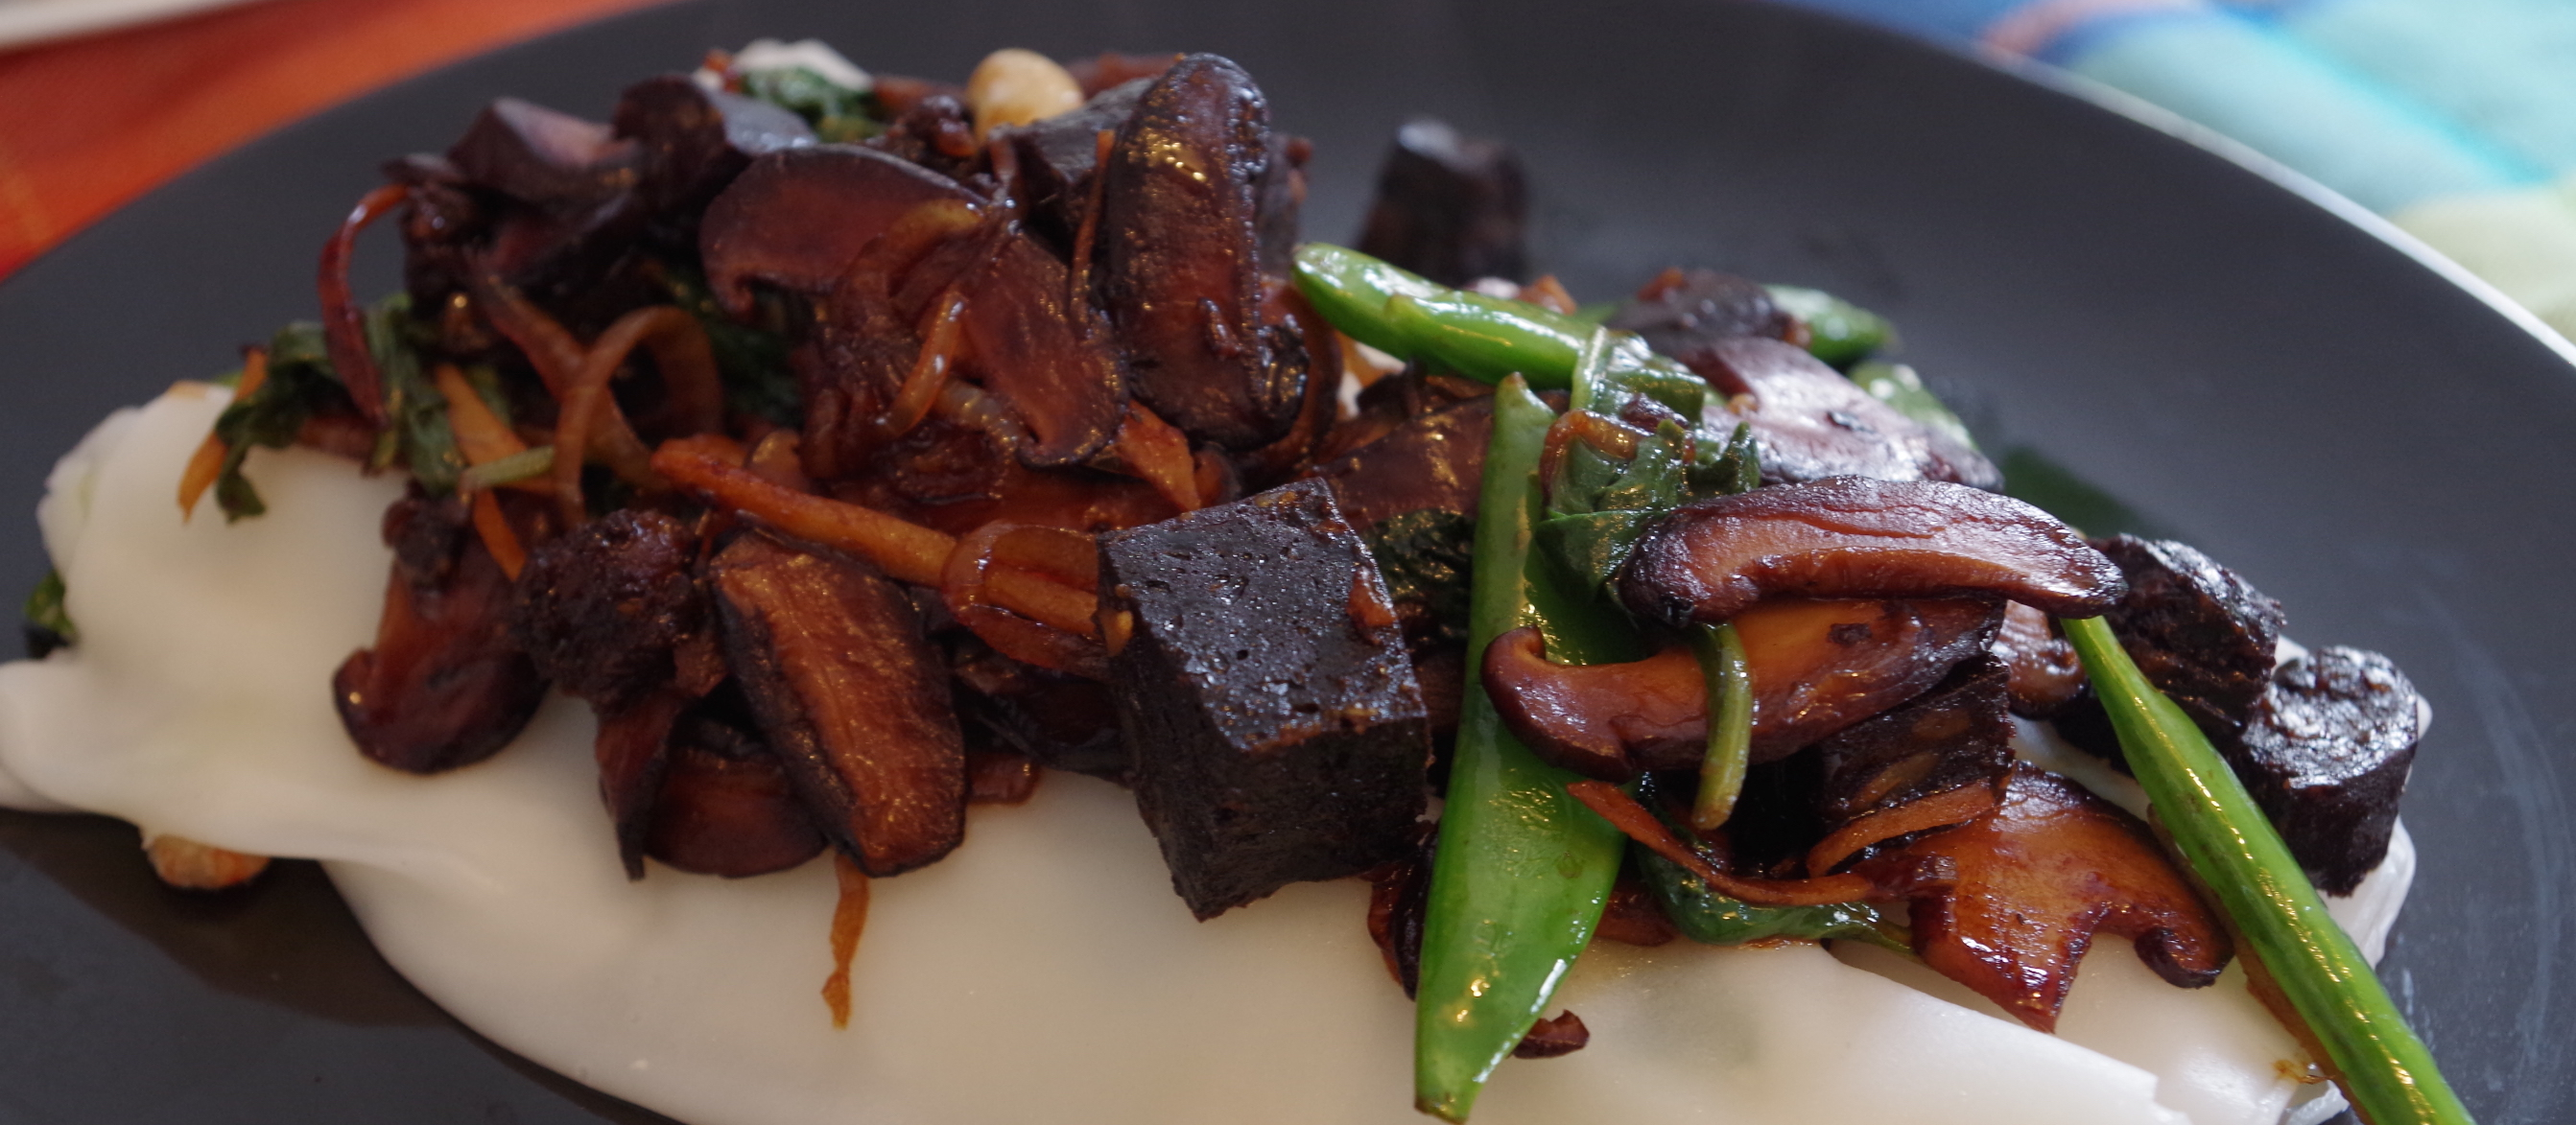
\includegraphics[width=\linewidth]{blackpuddingragout.png}
\end{figure*}

\section{Black pudding, pea, peanut, mushroom and spinach ragout}
\index{Mains!black pudding ragout}

This dish is a Scottish-Chinese hybrid, but it really works. The recipe comes from Peter Gordon at The Providores - a highly rated Kiwi restaurant in London.

\smallskip
\emph{200g black pudding
\\Peanut oil
\\Sesame oil
\\1 onion, peeled and thinly sliced
\\Big handful shitake mushrooms
\\Half thumb of ginger, julienned
\\50 ml mirin or 25ml rice wine vinegar
\\50 ml soy sauce
\\60 peanuts
\\100g spinach
\\100g peas
\\400g fresh rice noodles
}

\smallskip
Add the black pudding to a cold pan, and heat to medium high. Add a little oil if the black pudding isn't fatty. 
\\Once the black pudding is starting to go crispy, remove from the pan and add the oil, mushrooms and ginger.
\\When the onions have browned, add in the soy sauce and mirin (or rice wine vinegar) and cook till the pan goes dry.
\\Then add the peanuts, spinach and peas with a heavy splash of water.
\\Heat the noodles in the microwave by pouring on some water and covering with cling film.
\\To serve, add a little water if the ragout is dry, and place on the heated noodles.

%%%%%%%%%%%%%%%%%%%%%%%%%%%%%%%%%%%%%%%%%%%%%%%%%%%%

\begin{figure*}[h]
  \includegraphics[width=\linewidth]{breadcrumbpasta.png}
\end{figure*}

\section{Anchovy and breadcrumb pasta }
\index{Mains!Pasta}
\index{Pasta!Anchovy and breadcrumb}

A great store cupboard recipe - if you have bread, you probably have all the ingredients needed. With good quality olive oil it's an amazing dinner.

\smallskip
\emph{Spaghetti or linguine for three
\\1/3 cup extra-virgin olive oil, more as needed
\\12 anchovies, chopped
\\6 garlic cloves, minced
\\1/4 teaspoon red pepper flakes
\\1 cup good dried bread crumbs
\\2 egg yolks
\\1 tablespoon Asian fish sauce (optional)
\\1 teaspoon hot sauce, such as Tabasco, or to taste
\\1/2 cup roughly chopped parsley
\\ Peas, asparagus, or any quick cooking vegetable (optional)
\\Lemon wedges, for serving}

\smallskip
In a medium skillet over medium-high heat, warm oil. Add anchovies, garlic and red pepper flakes; cook until fragrant, 1 minute. Stir in bread crumbs and cook until golden, 2 to 3 minutes. Season liberally with black pepper, and a little salt if needed.
\\Bring a large pot of salted water to a boil. Add spaghetti and cook according to package instructions; drain well, reserving some of the pasta water (about 1/2 cup is plenty). If vegetables are being added, chuck them into the pasta a few minutes before the end.
\\In a large, preferably warmed bowl, stir together egg yolks, fish sauce, hot sauce and 2 tablespoons pasta water. Add hot pasta and toss well, adding more pasta water if the mixture looks dry or unevenly yellow. You want the yolk to evenly coat the pasta but you don't want it to be soupy. Add bread crumb mixture and parsley and toss well. Season with plenty of black pepper, and salt to taste. Drizzle pasta with more oil just before serving and serve with lemon wedges.

%%%%%%%%%%%%%%%%%%%%%%%%%%%%%%%%%%%%%%%%%%%%%%%%%%%%

\section{Phat thai}
\index{Mains!Phat thai}
\index{Noodles!Phat thai}

Phat thai and I have a weird relationship. Like how hollandaise becomes less appealing when you make it yourself (and see all the butter) - I can't seem to make good phat thai without a lot of oil. It's still a great, and easy dish to make - it just needs a lot of ingredients.

\smallskip
\emph{120g 2-3mm wide flat rice sticks
\\60ml fish sauce
\\60ml tamarind water
\\60g palm sugar
\\Pinch of chilli powder, to taste
\\80ml groundnut or vegetable oil
\\2 cloves of garlic, finely chopped
\\100g extra-firm tofu, chopped into small cubes
\\8 large prawns
\\2 large eggs, ready cracked
\\1 tbsp small dried shrimp
\\100g beansprouts
\\4 stalks Chinese chives, chopped
\\50g roasted peanuts, roughly chopped
\\Lime wedges, chilli flakes, fish sauce and sugar, to garnish}

\smallskip
Soak the rice sticks in cold water for about half an hour until pliable but al dente. Drain.
\\Meanwhile, make the sauce by combining the fish sauce, tamarind and palm sugar in a small pan. Heat gently to dissolve the sugar and taste. Add more of any of the ingredients as you wish. Season with chilli to taste. Set aside.
\\Lay out all the ingredients within easy reach of the hob in the order they'll be used. Put a wok on a high heat and add half the oil. Add the garlic, stir fry for a few seconds, then add the noodles and a splash of water. Stir fry until they're drying out, then add the sauce. Fry until they are almost soft enough to eat (they should be slightly chewy).
\\Push the noodles to the side of the wok and add the rest of the oil. Fry the tofu and prawns until the tofu is beginning to colour, then push to the side and add the eggs. Pierce the yolks and, when starting to set on the bottom, scramble.
\\Stir through the noodles, and add the radish, dried shrimp, beansprouts, chives and peanuts. Stir fry until well combined, then serve with the garnishes for people to add as they wish.

%%%%%%%%%%%%%%%%%%%%%%%%%%%%%%%%%%%%%%%%%%%%%%%%%%%%

\begin{figure*}[h]
  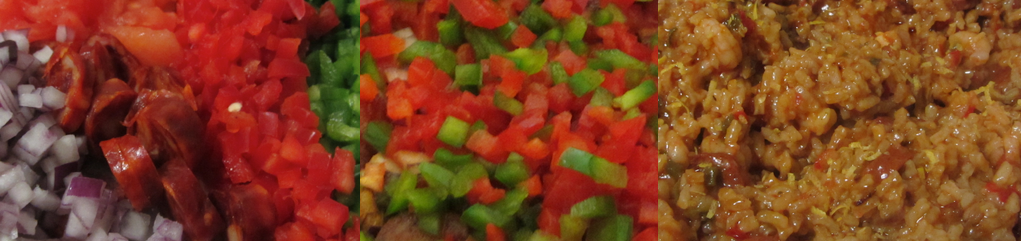
\includegraphics[width=\linewidth]{paella.png}
\end{figure*}

\section{Paella}
\index{Mains!paella}
\index{Rice!paella}
\index{Seafood!paella}

An easy dinner party dish as you can make it 90\% before hand, then just add the shellfish and reheat to serve.

\begin{marginfigure}%
  \includegraphics[width=\linewidth]{paellahigh.png}
\end{marginfigure}

\smallskip
\emph{250g tomatoes, with x in top\sidenote{Or half a tin of tomatoes}
\\100ml olive oil
\\6 chicken thighs\sidenote{You can easily omit either the chicken or prawns}
\\220g chorizo, sliced
\\1 onion, finely chopped
\\1 green pepper, finely chopped
\\1 red pepper, finely chopped
\\2 cloves garlic
\\1 1/2 tsp sweet paprika
\\1/2 tsp cayanne pepper
\\Large pinch of saffron
\\350g paella rice
\\1.2L stock
\\75g fresh peas
\\12 tiger prawns
\\3 tbsp chopped flat-leaf parsely leaves
\\Finely chopped zest and juice of one lemon
}

\smallskip
Boil the tomatoes for 10 seconds then skin and deseed.
\\Heat the oil in a large frying pan to medium and fry the chicken skin side down till dark brown with the chorizo.
\\Remove the chicken and add chorizo.\sidenote{I like to blend 1/3 of the chorizo so it melts into the paella, but that's completely optional and probably heresy.}
\\Soon after, add the peppers and garlic and fry for 3 minutes.
\\Add the spices and rice.
\\After a few minutes, once the rice starts to go clear, add the stock and tomatoes and bring to the boil.\sidenote{If you deheaded the shrimp, I like to add it to the stock while it's heating (discard before adding to the paella).}
\\Turn the heat to low and simmer for 15 minutes with the lid off.
\\Then add back the chicken, with the prawns and peas, and cook for 15 more minutes.\sidenote{If the prawns are large, turn them once by hand to make sure they cook through.}
\\Squeeze over a lemon and sprinkle with zest and juice.

%%%%%%%%%%%%%%%%%%%%%%%%%%%%%%%%%%%%%%%%%

\begin{figure*}[h]
  \includegraphics[width=\linewidth]{porkpie.png}
\end{figure*}

\section{Pork and Prune Pie}
\index{Mains!pork pie}
\index{Pie!pork \& prune}
\index{Pork!\& prune}
\index{Stew!pork and prune}

This is a super easy, and tasty stew that doesn't have to served in a pie. The fruit makes it quite rich, so in lieu of pastry it needs something like mashed potatoes as a side. Serves at least four.

\smallskip
\emph{400g diced pork
\\2 tbsp flour
\\2 tbsp oil
\\1 onion, diced finely
\\4 apples, peeled and chopped
\\2 cloves garlic
\\2 cups apple juice or cider
\\150g pitted prunes
\\Shortcrust pastry packet
\\4 tbsp milk}

\smallskip
Toss pork in flour and fry until lightly brown, then put aside.
\\Fry onion, garlic and apple for 3 minutes.
\\Add apple juice or cider to deglaze, then add the prunes.
\\Cook on low for about an hour, then let it cool with the pan off the heat.
\\When cold (or at least cool-ish), make pie and glaze pastry with milk.

%%%%%%%%%%%%%%%%%%%%%%%%%%%%%%%%%%%%%%%%%

\section{Moroccan lamb}
\index{Mains!Moroccan lamb}
\index{Lamb!Moroccan stew}
\index{Stew!Moroccan}

\emph{1 kg lamb in 4 cm cubes
\\2 onions
\\15g butter
\\2 tbsp oil
\\1 tsp black pepper
\\1 cinnamon stick
\\1 1/2 tbsp honey
\\2 tsp ground ginger
\\2 tsp ground cumin
\\1 1/2 tbsp ground cinnamon
\\200g dried apricots
\\200g prunes
\\2 long strips lemon rind}

\smallskip
Remove all fat from lamb then sear in butter, and remove.
\\Add spices and onion and fry till soft.
\\Add lamb back in, cover and simmer for an hour.
\\Remove lid, add lemon rind, honey, cinnamon, and fruit and simmer for 30mins with the lid off.\sidenote{
Becareful of it suddenly thickening thanks to the prunes, as it will stick.}


%%%%%%%%%%%%%%%%%%%%%%%%%%%%%%%%%%%%%%%%%
\chapter{Vegetarian curries}
%%%%%%%%%%%%%%%%%%%%%%%%%%%%%%%%%%%%%%%%%

\section{Carrot sambal}
\index{Vegetarian curries!carrot sambal}
\index{Salads!carrot sambal}
\index{Carrot!Sambal}

\begin{marginfigure}%
  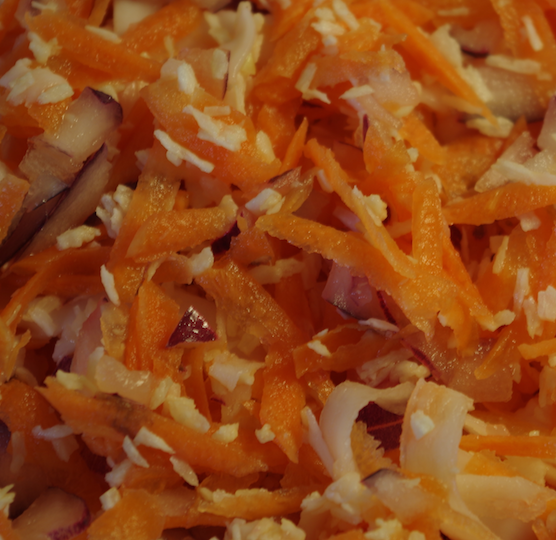
\includegraphics[width=\linewidth]{carrotraita.png}
\end{marginfigure}

Super simple, light and refreshing. Letting it sit in the fridge softens the coconut a lot, and changes the dish substantially. It's best to season just before eating to keep the carrots firmer.

\smallskip
\emph{2 large carrots, grated
\\1 small red onion, diced
\\1 chilli, diced
\\2 big splashes lime juice
\\1/2 cup desiccated coconut
\\Salt and pepper to taste}

\smallskip
Mix everything. Best served slightly chilled after a few hours in the fridge.

%%%%%%%%%%%%%%%%%%%%%%%%%%%%%%%%%%%%%%%%%

\index{Vegetarian curries!fried potatoes}
\index{Potato!fried}

\section{Fried potatoes}
\emph{1/2kg boiled potatoes
\\1/4kg onions
\\5 curry leaves
\\2 tbsp Maldive fish (optional)
\\1/4 tsp tumeric
\\2 tbsp chilli
\\4 tbsp olive oil
\\salt to season
}

%EXAMPLE MARGIN FIGURE
\begin{marginfigure}%
  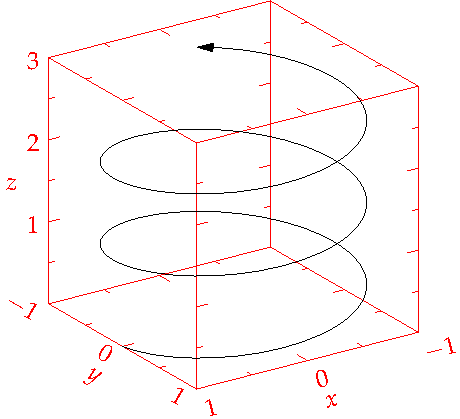
\includegraphics[width=\linewidth]{helix}
\end{marginfigure}

\smallskip
Mix the potatoes, tumeric and salt.
\\Heat the oil till hot and fry chilli and curry leaves.
\\Add onion and fry till golden brown.
\\Add the potatoes and toss till hot.

%%%%%%%%%%%%%%%%%%%%%%%%%%%%%%%%%%%%%%%%%

\section{Curried carrots}
\index{Vegetarian curries!curried carrots}\index{Carrot!curried}
\emph{Carrots\sidenote{Bill gives no measurments here - and you don't need them. This is a super simple side dish to go alongside a chicken curry or similar.}
\\Lemon juice
\\Sugar
\\Olive oil
\\Black or white mustard seeds
}

\smallskip
Grate carrots and dress with lemon juice and sugar.
\\Heat a little oil and mustard seeds, as soon as they pop pour the mustard over the carrots and mix.

%Example full width picture
\begin{figure*}[h]
  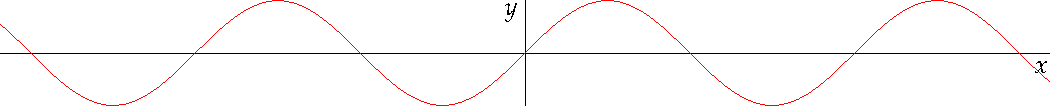
\includegraphics[width=\linewidth]{sine.pdf}%
\end{figure*}


%%%%%%%%%%%%%%%%%%%%%%%%%%%%%%%%%%%%%%%%%

\section{Spinach and coconut cream}
\index{Vegetarian curries!spinach \& coconut cream}\index{Spinach!coconut cream}

One of my favourite side dishes. It's super easy to make and the spinach soaks up all the coconut sauce.

\smallskip
\emph{Packet spinach, roughly chopped
\\Medium onion, finely chopped
\\Oil
\\2 tbsp mustard seeds
\\1 cup coconut milk
\\Salt to season
}

\smallskip
Fry mustard seeds till they pop.
\\Add onions and fry till soft.
\\Add turmeric and salt.
\\Add coconut milk, when thickness as you want add spinach.
\\Season and eat.

%%%%%%%%%%%%%%%%%%%%%%%%%%%%%%%%%%%%%%%%%
%Example text width image

\section{Leek curry with cashew nuts}
\index{Vegetarian curries!leek and cashew}
\index{Leek!cashew nuts}
\emph{1 1/2 cashew nuts, soaked in water for at least 2 hours
\\2 or 3 leeks
\\1 onion
\\2 tbsp mustard seeds
\\1/2 tsp turmeric
\\3 cloves garlic, sliced
\\10 curry leaves
}

\smallskip
Fry onions, garlic and curry leaves until soft.
\\Add mustard seeds and fry till seeds start to pop.
\\Add turmeric, seeds and nuts.
\\Add some water, white wine or chinese wine to steam.

%%%%%%%%%%%%%%%%%%%%%%%%%%%%%%%%%%%%%%%%%

\section{Pumpkin curry}
\index{Vegetarian curries!pumpkin curry}
\index{Pumpkin!curry}
\emph{1 cup red lentils
\\700g pumpkin peeled, chopped, and roasted.
\\1 tbsp oil
\\1 onion
\\Fresh ginger to taste
\\2 cloves garlic, crushed
\\1/4 cop Korma curry paste
\\1 tbsp mustard seeds
\\400ml coconut cream
\\Spinach\sidenote{Optional, can also use silverbeet, peas, or any other green vegetable.}}

\smallskip
Cook lentils in a large pot of water until tender (about 10 minutes), then drain.
\\Heat oil and fry onion, garlic and giner till cooked. 
\\Add curry paste and seeds and cook until fragrant.
\\Add lentils, pumpkin and coconut cream and cook until boils.
\\Add green vegetable and cook until tender.
\\Serve with rice.

%%%%%%%%%%%%%%%%%%%%%%%%%%%%%%%%%%%%%%%%%
\chapter{Nana's curries}
%%%%%%%%%%%%%%%%%%%%%%%%%%%%%%%%%%%%%%%%%

\section{Nana's brinjal}
\index{Nana's!brinjal}
\index{Eggplant!Nana's brinjal}
\index{Vegetarian curries!Nana's brinjal}

Nana was known for creating the three greatest dishes in the culinary world (marrow bone mutton curry, Nana's rolls \& Nana's brinjol). The original eggplant dish required the vegetable to be fried. If you fry - the dish will be incredible, but it will soak up at least 250mls of oil. Hence the slightly more waistline friendly recipe below.

\smallskip
\emph{3-4 Brinjal (eggplant)
\\1 tbsp mustard seeds
\\a few heavy splashes of oil
\\3 onions, diced or sliced
\\1 tsp salt
\\1 chillies, finely diced
\\2 tsp tumeric
\\1 stem curry leaves
\\1 tin coconut milk}

\smallskip
Preheat the oven to 200\celsius 
\\Dice the brinjal and pour over the oil. Tip into an overproof tray and cook for 40 minutes, or till brown.
\\In a fry pan, fry the mustard seeds in a little oil.
\\Once the seeds start popping, add the onions, chilli, tumeric and curry leaves and fry till it starts to get brown.
\\Once browned, add the coconut milk, and cook on medium with the lid off for for 15 minutes.  
\\Add the aubergine back in, and serve.

\begin{figure}
  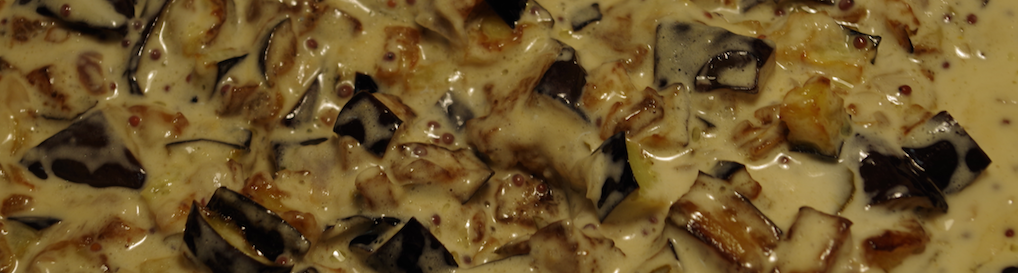
\includegraphics{eggplantcurry.png}
%  \checkparity This is an \pageparity\ page.%
  %\zsavepos{pos:textfig}
\end{figure}

%%%%%%%%%%%%%%%%%%%%%%%%%%%%%%%%%%%%%%%%%

\section{Curried vegetables}
\index{Vegetarian curries!Nana's}
\index{Nana's!Curried vegetables}

\emph{Any diced vegetables\sidenote{Potatoes, cauliflower, courgettes, carrots, etc.}
\\1/2 onions finely chopped
\\1 chilli sliced diagonally
\\1 stem curry leaves chopped
\\1 tsp mild indian curry powder
\\1/2 tsp turmeric
\\1 tsp garlic
\\1 tsp cumin seeds
\\1 ripe tomato, skinned and diced
\\1 tbsp water or stock
\\Salt
\\Oil for frying}

\smallskip
Gently fry onions, curry leaves, cumin seeds and chillies.\sidenote{Stir often during this step.}
\\Add potatoes and water and simmer.
\\Add other vegetables in order they need to cook.
\\Add tomatoes when almost cooked, the tomato forms the sauce.

%%%%%%%%%%%%%%%%%%%%%%%%%%%%%%%%%%%%%%%%%

\section{Nana's dahl}
\index{Nana's!dahl}
\index{Vegetarian curries!Nana's dahl}

This dish can be served a bit runny, or quite dry. I prefer it pretty dry, and with the dahl completely broken down, which can be achieved by cooking it for an extra hour or so.

\smallskip
\emph{1 1/2 cups red lentils
\\1/2 tsp turmeric
\\1 tsp salt
\\2 small green chillies, finely diced
\\5 tbsp ghee or butter
\\2 medium onions, finely chopped
\\1 tbsp fresh ginger, grated
\\2 large finely chopped tomatoes
\\1 tsp mustard seeds
\\1 tsp fennel seeds
\\1 tsp nigella seeds
\\1/2 tsp fenugreek seeds
\\4 curry leaves
\\2 small red chillies
\\2 cloves garlic, chopped}

\smallskip
Fry onions in 3 tbsp ghee. 
\\When beginning to brown, add ginger and tomatoes, cooking till the tomatoes are reduced.
\\Add dahl and 5 cups water and bring to the boil, with turmeric, salt and green chillies.
\\Simmer for 50 minutes, stirring and adding water if it gets thick enough to burn.
\\As the lentils begin to dissolve, fry the seeds, garlic and the whole red chillies till is begins to brown. 
\\Combine the spices and the dahl, and serve.\sidenote{Add one tin coconut milk to Nana's dahl. Stir in spinach, serve with half boiled eggs and coriander on top}

%%%%%%%%%%%%%%%%%%%%%%%%%%%%%%%%%%%%%%%%%

\section{Nana's chicken curry}
\index{Nana's!chicken curry}
\index{Meat curries!Nana's chicken}
\index{Chicken!Nana's curry}

A relatively easy curry. I like it with the skin removed, although you could try browning the chicken to make the skin more appealing.

\smallskip
\emph{1.25 kg chicken chopped
\\2 onions, finely chopped
\\2 chillies, chopped
\\10 curry leaves, chopped
\\2 tbsp Jaffna curry powder
\\1 tsp cinnamon, cloves, cardamon and salt
\\200ml coconut cream
\\1 clove garlic
\\2 tbsp chopped ginger
\\2 tsp fenugreek, cumin and fennel
\\Juice of one lemon
\\Salt
\\Oil}

\smallskip
Coat meat with curry powder and salt. 
\\Marinate for 24 hours in the fridge.
\\Gently fry onions, curry leaves, and chillies. When clear, add the spices and fry till brown.
\\Add the garlic and ginger and fry for 5 minutes.
\\Add meat and fry gently for 10 minutes.
\\Add the coconut cream and simmer gently for 20 minutes or until tender.
\\Add lemon juice just before serving.

%%%%%%%%%%%%%%%%%%%%%%%%%%%%%%%%%%%%%%%%%
\chapter{Meat curries}
%%%%%%%%%%%%%%%%%%%%%%%%%%%%%%%%%%%%%%%%%

\section{Lamb curry}
\index{Lamb!curry}
\index{Meat curries!Lamb}

Nana's lamb/mutton marrow bone curry is one of my favourite dishes. In Sri Lanka mutton usually means goat, but lamb is often substituted in New Zealand. While this isn't Nana's recipe - it's still worth seeking out marrow bones for the curry.

Jaffna curry powder is dark roasted, and while optional, without it the curry has a very different taste.

\smallskip
\emph{3 tbsp ghee or butter
\\1 kg bone in lamb, diced
\\1 tin tomatoes
\\200ml stock
\\2 chillies, chopped
\\10 curry leaves, chopped
\\1 tbsp Jaffna curry powder (optional)
\\2 tbsp fennel, cinnamon, cumin, coriander, fenugreek, pepper, all ground, cardamon
\\5cm ginger
\\2 red onions, diced
\\10 cloves garlic
\\1 big bunch coriander}

\smallskip
Pre-heat oven to 170\celsius.
\\Put everything from the chillies, to the garlic in a food processor. Add half the coriander, then blend.
\\In an oven proof dish, fry the paste in the butter till it goes brown.
\\Add the tomatoes and the stock, cover in foil, and place in the oven for 1.5 hours.
\\Remove the foil and return to the stove.
\\Add the lamb, and cook for 1.5 hours, with the lid off for about half that time.

%%%%%%%%%%%%%%%%%%%%%%%%%%%%%%%%%%%%%%%%%

\begin{figure*}[h]
  \includegraphics[width=\linewidth]{britcurry.png}%
\end{figure*}

\section{Chicken curry (Scottish style)}
\index{Chicken!curry}
\index{Meat curries!Chicken}

Similar to a chicken tikka masala, a Glaswegian curry, but without the sweetness or food colouring.

\smallskip
\newpart{For curry:}
\\\emph{4 skinless chicken thighs or breasts
\\2 onions
\\Thumb-sized piece of fresh ginger
\\1/2 bunch fresh coriander
\\1 fresh red chilli
\\1/2 tin of chopped tomatoes
\\400g tin coconut cream
\\Handful of flaked almonds, to serve
\\1 lemon, to serve}
\\\newpart{For spice paste:}
\\\emph{2 cloves of garlic
\\Thumb-sized piece of fresh ginger
\\1 teaspoon cumin seeds
\\1 teaspoon coriander seeds
\\1 teaspoon cayenne pepper
\\1 teaspoon sugar
\\2 teaspoons garam masala
\\1/2 teaspoon sea salt
\\2 tablespoons groundnut oil
\\2 tablespoons tomato puree
\\Small bunch of fresh coriander
\\1/2 tablespoon desiccated coconut
\\2 tablespoons ground almonds}

\smallskip
To make the curry paste, halve, deseed and roughly chop the chillies, then peel the garlic and ginger. 
\\Put a frying pan over a medium-high heat and add the cumin and coriander seeds. Lightly toast for a few minutes, or until golden brown and smelling delicious, then remove from the heat. 
\\Add the toasted spices to a pestle and mortar and grind until fine, or put them in a food processor and whiz to a powder. 
\\Once you've ground them, add the toasted spices to a food processor along with the remaining paste ingredients and whiz to a smooth paste, then put to one side.
\\Slice the chicken lengthways into 2cm strips. 
\\On a clean chopping board, peel, halve and finely slice the onions. Peel and finely slice the ginger, then pick the coriander leaves and put to one side, finely chopping the stalks along with the chilli.
\\Place a large casserole pan over a medium-high heat and add a couple of lugs of oil. Once hot, add the onions, chilli, ginger and coriander stalks, then cook for around 10 minutes, or until softened and lightly golden. 
\\Add the chicken and roughly 140g of the tikka masala paste, stirring well so everything is nicely coated. Season with salt and pepper, add the tomatoes and coconut milk (save the rest for another day), then bring everything to the boil.
\\Turn the heat down to medium-low, cover and simmer for 20 minutes, then take the lid off and cook for further 5 minutes, or until the meat is tender and the sauce has reduced, stirring occasionally. 
\\Divide the curry between bowls, sprinkle over the almonds and coriander leaves. Serve with fluffy rice, a dollop of yoghurt and lemon wedges for squeezing over.

%%%%%%%%%%%%%%%%%%%%%%%%%%%%%%%%%%%%%%%%%

\section{Thai chicken curry}
\index{Meat curries!Thai chicken}
\index{Chicken!Thai curry}

\emph{2 tbsp oil
\\1 medium onion, sliced
\\2 cloves garlic, chopped
\\3 tbsp Thai red curry paste\sidenote{You can use red,green or even a penang curry paste here.}
\\3 kaffir lime leaves, chopped
\\500g minced chicken\sidenote{Or diced chicken or beef. If adding fish, add with the fish sauce and briefly simmer till cooked.}
\\1 cup coconut cream
\\1 cup chicken stock
\\1/2 cup crunchy peanut butter
\\2 tbsp fish sauce
\\1 tsp each salt and sugar
\\3 tbsp coriander, chopped
\\1-2 cups sliced or diced vegetables (zucchini, cauliflower, broccoli, carrots, beans, peas)
\\Spring onions or roasted peanuts}

\smallskip
Heat the oil, add the onion and garlic and cook.
\\Stir in the curry paste and lime leaves.
\\Add minced chicken, cook till meat is white.
\\Add coconut cream/stock and stir in peanut butter and cook for 8 minutes.
\\Add fish sauce, salt and sugar, serve when vegetables are cooked.

%%%%%%%%%%%%%%%%%%%%%%%%%%%%%%%%%%%%%%%%%
\chapter{Dessert}
%%%%%%%%%%%%%%%%%%%%%%%%%%%%%%%%%%%%%%%%%

\begin{figure*}[h]
  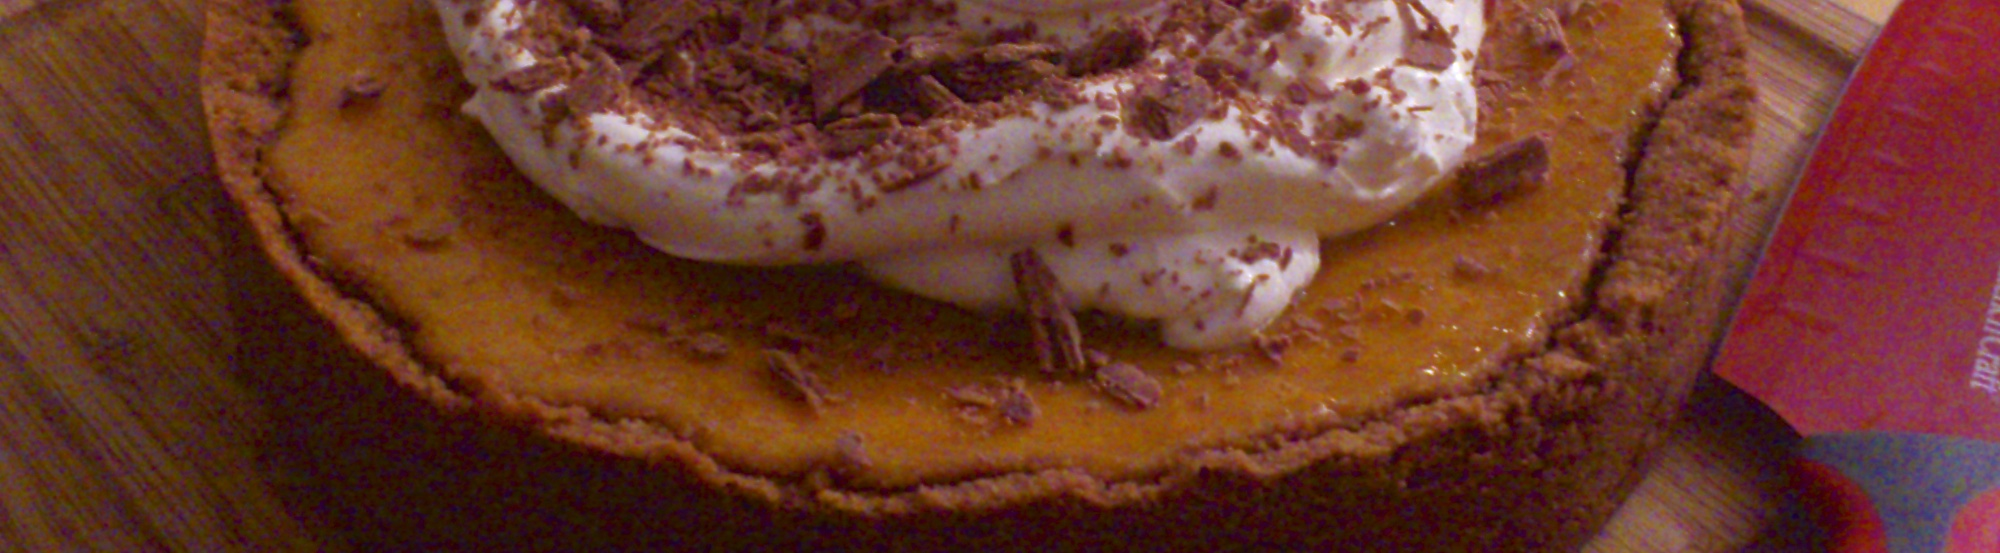
\includegraphics[width=\linewidth]{pumpkinpie.jpg}%
\end{figure*}

\section{Pumpkin pie}
\index{Dessert!pumpkin pie}
\index{Pie!pumpkin}
\index{Pumpkin!pie}

\emph{14 ounces chocolate wafers, finely ground
\\3/4 cup (1 1/2 sticks) unsalted butter, melted
\\1 pumpkin, roasted and blended.\sidenote{
You can also use 3 sweet potatoes, or 2 squashes. Just make sure to roast, not boil, and add a little water when you puree.}
\\1 (14 ounce) can sweetened condensed milk
\\1/2 lemon, juiced
\\5 tablespoons salted butter, melted
\\3 1/2 tablespoons light brown sugar
\\2 eggs
\\1 tablespoon vanilla extract
\\2 teaspoon ground cinnamon
\\1/2 teaspoon nutmeg
\\Sweetened whipped cream:
\\1 cup heavy cream
\\1/2 cup superfine sugar
\\1/2 teaspoon vanilla extract
\\Cadbury flake
}

\smallskip
Preheat oven to 170\celsius
\\\newpart{For crust:} 
\\In a large bowl mix together the chocolate wafer crumbs and melted butter until fully incorporated. Press the mixture into a pie dish or tart shell, pressing both evenly on the bottom and up the sides. Place onto a baking sheet and then into the refrigerator until ready to use.
\begin{marginfigure}%
  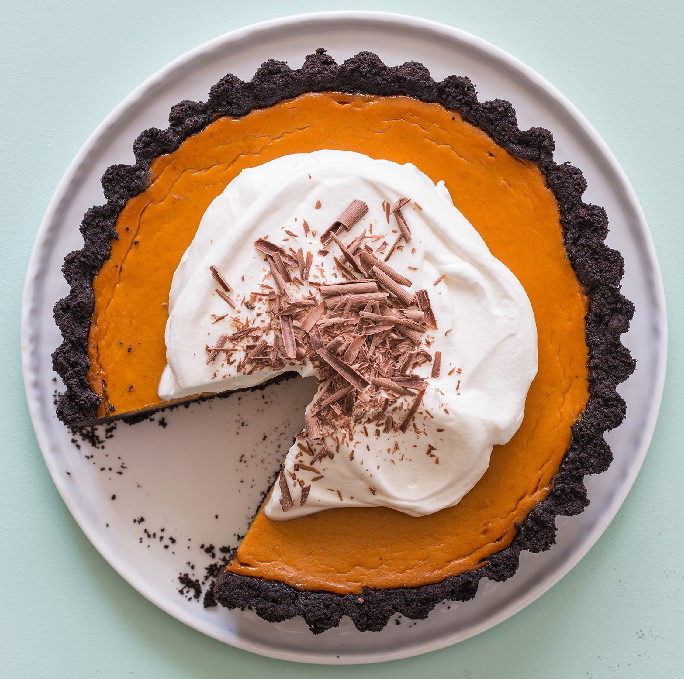
\includegraphics[width=\linewidth]{pumpkinpiesquare.png}
\end{marginfigure}
\newpart{For filling:} 
\\Place pumpkin puree in a bowl and add the remaining filling ingredients. Stir together until fully incorporated and no lumps remain. Pour the filling into the prepared crust and carefully set into the lowest rack of the oven. Bake for 55 to 70 minutes or until the filling has set, but is slightly loose in the middle.
\\Allow pie to cool completely, about 2 hours.
\\\newpart{For sweetened cream:} 
\\Pour cream, sugar and vanilla extract into a mixing bowl and beat together using an electric hand mixer until stiff peaks form.
\\Generously top pie with whipped cream and finish with the crumbled flake to serve.

%%%%%%%%%%%%%%%%%%%%%%%%%%%%%%%%%%%%%%%%%

\section{German mess}
\index{Dessert!German mess}

Apparently it's called "Raspberry Dream" in Germany. Really, it's an Eton Mess. The substitution of cream for the cheeses makes it taste a lot less creamy.

Ingredients for 6 portions:

\emph{200g meringue
\\500g frozen raspberries
\\500g mascarpone (or instead: 250g sour cream and 250g soft cheese)
\\250g quark
\\vanilla essence 
}

\smallskip
Mix mascarpone, quark, and vanilla.
\\Break meringue in pieces (not too small).
\\Fill mascarpone mix, raspberries and meringue in a bowl in layers.
\\Leave for 3-4 hours in the fridge.

\begin{figure*}[h]
  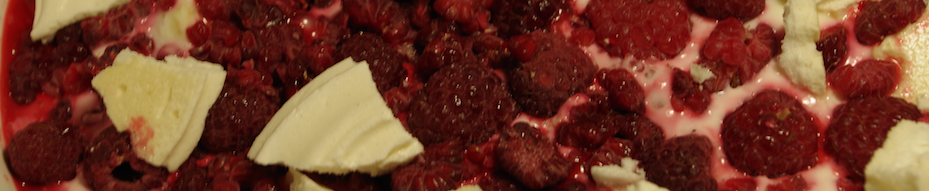
\includegraphics[width=\linewidth]{germanmess_banner.png}%
\end{figure*}


\backmatter

%\bibliography{sample-handout}
%\bibliographystyle{plainnat}


\printindex
\printindex[recipe][Recipe list]


\end{document}

